\documentclass[12pt]{article}
\usepackage[letterpaper,margin=1.25in]{geometry}
\usepackage{amsmath,amssymb,amsthm}
\usepackage{setspace}
\usepackage{booktabs}
\usepackage{graphicx}
\usepackage{enumitem}
\usepackage[hidelinks]{hyperref}
\setstretch{1.33}
\setlength{\parskip}{3pt}
\setlist{itemsep=2pt,topsep=4pt}
\setlist[itemize]{label=$\bullet$}
\emergencystretch=2em

\newtheorem{theorem}{Theorem}
\newtheorem{proposition}{Proposition}
\newtheorem{corollary}{Corollary}
\newtheorem{result}{Result}
\theoremstyle{definition}
\newtheorem{assumption}{Assumption}
\theoremstyle{remark}
\newtheorem*{inwords}{In words}

\newcommand{\E}{\mathbb{E}}
\newcommand{\R}{\mathbb{R}}
\newcommand{\mut}{\tilde\mu}
\newcommand{\OAref}[1]{\ref{#1}}
\newcommand{\cA}{\mathcal{A}}
\newcommand{\cT}{\mathcal{T}}
\newcommand{\cF}{\mathcal{F}}
\newcommand{\cG}{\mathcal{G}}
\theoremstyle{plain}
\newtheorem{alemma}{Lemma}[section]
\newtheorem{atheorem}[alemma]{Theorem}
\newtheorem{aproposition}[alemma]{Proposition}
\newtheorem{acorollary}[alemma]{Corollary}
\theoremstyle{definition}
\newtheorem{adefinition}[alemma]{Definition}
\newtheorem{aremark}[alemma]{Remark}

\title{Rational Foreclosure:\\[2pt] \Large Hope as an Economic Variable}
\author{Ryan Lester\\[2pt] \normalsize University of Houston\\ \normalsize\texttt{rslester@cougarnet.uh.edu}}
\date{November 2026}

\begin{document}
\maketitle
\thispagestyle{empty}

\begin{abstract}
\noindent A generation of young workers stands accused of quiet quitting: showing up, doing the job, and declining the long hours their parents treated as the price of getting ahead. The standard diagnosis is weak self-control; the standard cure is a nudge toward persistence. The diagnosis can be backwards. A loss-averse agent measures her wealth against a social benchmark that moves at random, such as local house prices, and may stop keeping score for good. She persists near the benchmark, sacrifices less as she falls behind, and quits at a precise threshold strictly below it. A more volatile benchmark makes her hold on longer; one that steadily outruns her resources makes her quit sooner. Holding her in the race past her threshold has an exact, strictly positive welfare cost. Because the benchmark is shared, one shock moves a whole cohort toward its threshold at once, and a runaway benchmark becomes a disengaged workforce.
\end{abstract}

\noindent\textbf{Keywords:} optimal stopping, reference dependence, aspirations, loss aversion, real options, behavioral welfare, quiet quitting.\\
\textbf{JEL:} D15, D81, D91, I31, J22.

\newpage
\setcounter{page}{1}

\section{Introduction}\label{sec:intro}

When I trained as a Navy drill instructor, I kept falling out of one conditioning run. After the third failure I told my mentor that if I only knew how long the run was, I could finish it. She told me: twelve laps. At the next session I paced myself, planned my effort, and stayed with the group the whole way. My legs had not changed. What changed was that I could see the finish line.

Military training often teaches the reverse lesson on purpose. David Goggins, a former Navy SEAL, describes instructor-led runs on which ``we knew the start and end point,'' and instructors who, hearing the class relax as the end came near, would ``go right on past the end point''; when they did, ``everybody stopped talking'' (Goggins n.d.). His creed inverts the twelve laps: ``When the ending is unknown and the distance is unknown, that's when you know who [\ldots] you are.'' Years later I ran the same exercise with my own recruits. I told them how far we would run, reached it, and kept running for another thirty minutes. About half visibly deflated; some fell, and many simply started walking. Same legs, same lungs. The finish line had moved.

The pattern has a laboratory counterpart. Richter (1957) placed wild rats in water from which there was no escape. All 34 died within one to fifteen minutes, and Richter wrote that they ``seem literally to `give up.'\,'' Wild rats that had first been held and released, and briefly immersed and taken out, learned that the situation was ``not actually hopeless,'' and then swam ``just as long as domestic rats or longer,'' which in his experiments was 40 to 60 hours. What separated the two groups was not strength. It was whether an end could come.

The three stories share one object, a reference point, and two questions about it: can the chaser see it, and does it move? This paper studies the economic version: when it is rational to stop chasing a target that moves at random, and what it costs to be talked out of stopping.

The paper makes three contributions. First, it solves exactly the problem of a loss-averse agent who chases a benchmark that moves at random and may stop keeping score for good. She quits at a threshold strictly below the benchmark, and the threshold has an explicit lower bound. No transversality condition is imposed on her plans. Second, it shows that a more volatile benchmark delays quitting, which gives hope an exact value, and that a benchmark that runs away hastens it. The volatility result is proved whenever the value of staying is convex in her standing, which covers every case in which gains and losses weigh equally, and it holds numerically in every other case computed. Third, it gives an exact expression for the cost of keeping someone in the race past her own quitting point. The volatility prediction is what separates this model from bias-based, aspirations and fixed-reference accounts of giving up, none of which has a target that moves on its own (Section~\ref{sec:why}). Because the benchmark is shared, the same solution turns an observable benchmark into the share of a cohort that has stopped keeping score.

Many of the targets people chase in economic life move. The house a young household hopes to buy, the salary that marks a career as on track, and the median firm in an industry all drift and jump for reasons the chaser does not control (Cai and Shefrin 2018 document the firm version; Section~\ref{sec:model} returns to it).

The question has a live application. Young workers have not stopped working: 80.7 percent of Americans aged 25 to 54 are employed (Bureau of Labor Statistics 2026b). They have stopped grinding. Gallup estimates that at least half of U.S. workers are ``quiet quitting,'' doing their jobs without reaching beyond them (Harter 2022). Engagement has fallen from 36 percent in 2020 to 31 percent in 2025, about 8 million fewer engaged workers (Harter 2026), and the long-hours tail of the workweek has pulled back, most among prime-age men with degrees who already worked long hours (Lee, Park and Shin 2023).

Meanwhile the finish line has moved. Since 1979, real GDP per person in the United States has more than doubled, while the real median weekly pay of full-time workers has risen 13 percent (Bureau of Economic Analysis 2026; Bureau of Labor Statistics 2026a). Pay has kept up with prices in general. It has not kept up with the economy it helps produce, or with the things people measure themselves against. A typical home now costs about five times a typical household income, against a traditional benchmark of three (Joint Center for Housing Studies 2025). The median first-time home buyer is 40 years old, up from 29 in 1981 (National Association of Realtors 2025). A generation ago, a young worker could look one cohort ahead and see the laps. About 90 percent of Americans born in 1940 grew up to earn more than their parents; among those born in the 1980s, half did (Chetty et al.\ 2017). The usual reading of the disengagement is a generational loss of grit. The model offers another: its agent can stay in the race while sacrificing very little for it, waiting to see whether the benchmark comes back.

The stakes are not only private. Gallup puts the cost of disengagement to U.S. employers at about 1.9 trillion dollars in lost productivity in 2023 (Bloomberg Law 2024), and the cost worldwide at about 10 trillion dollars a year (Gallup 2026). Section~\ref{sec:aggregate} takes the model from one person to a cohort and sets the evidence at that scale beside it.

That usual reading has a theory behind it. In the planner-doer model of Thaler and Shefrin (1981), a far-sighted planner and a myopic doer share one mind, and abandonment of a long-run goal is the doer winning. The policy response is to strengthen the planner: commitment devices, defaults, reminders, and other nudges toward persistence (Thaler and Sunstein 2008). That response is right when the doer is the one quitting. It is wrong when the planner is the one quitting, because then the nudge overrides a correct plan. Observed disengagement cannot tell the two apart. A model in which the planner's own optimal policy includes an exit rule can.

\paragraph{What this paper is for.} It does not argue that people should give up on their goals, or that everyone who stops striving is right to. Its claim is narrower and, for policy, more useful. When many people disengage at once, the cause may be the path of a benchmark they share rather than a failure of will, and then the remedy lies in the benchmark. A workforce that has stopped grinding costs the economy as well as the people in it, and pushing harder on individuals will not recover the loss if the finish line keeps moving. It is written for economists and for the policymakers, central banks included, who track the benchmarks people chase and can sometimes change how fast those benchmarks pull away. A companion planning tool, described under Data and code, puts the model to work with current data for the nation, every state and county, and large cities.

\subsection{What the model does}

The agent has wealth that grows at a known rate and a benchmark, the reference level she measures herself against, that grows on average but also moves at random. While she is in the race, she enjoys consumption and also feels the gap between her wealth and the benchmark, with shortfalls weighted more heavily than leads, as in Kahneman and Tversky (1979). At a time of her choosing she can leave the race: she stops scoring herself against the benchmark for good, and from then on cares only about consumption. Leaving is irreversible. She chooses how much to consume and when to leave.

Two features carry the analysis. The benchmark moves at random, so the gap can close or widen on its own. And leaving removes the comparison but not the material goal: after exit she still consumes and still values wealth, and what she gives up is the scorecard. While she is in the race, she consumes less than she otherwise would, because every dollar saved improves her standing. That forgone consumption is the model's measure of the grind.

\paragraph{The argument without symbols.} Picture someone measuring her savings against the price of the home she wants. While she is close to it, the race is worth the sacrifice, and she saves hard. As the price pulls away, the race is worth less, and she sacrifices less for it. Below a certain point the race is worth nothing, and she does best to stop keeping score; the model locates that point exactly. How far behind she should be willing to fall depends on how the price moves. If it swings around, it may swing back toward her, and that chance is worth waiting for. If it climbs steadily away, there is nothing to wait for. And someone who pushes her to keep chasing after she has reached her stopping point is not helping her. The harm from a small push is small, and it grows quickly as the push gets bigger.

\subsection{Results}

The proved results:\footnote{Theorems are the main proved results and Propositions the supporting ones; anything labeled Result is numerical, with the range checked stated.}

\begin{enumerate}[label=(\roman*)]
\item \emph{The problem collapses to one dimension} (Proposition~\ref{prop:reduction}). Everything that matters about the agent's position is summarized by one number, the ratio $x=W/R$ of her wealth $W$ to the benchmark $R$. Plans face no transversality condition, the technical restriction most such models place on how fast wealth may be run down, and none is needed.
\item \emph{Exit is a threshold rule, and the threshold is pinned down} (Theorem~\ref{thm:main}). The agent quits exactly when $x$ falls to a threshold $x^*$, which lies strictly below par ($x=1$, wealth equal to the benchmark) and above an explicit bound $\bar x$. Her extra saving for the race vanishes as she reaches $x^*$, so consumption does not jump when she quits.
\item \emph{Volatility delays exit} (Theorem~\ref{thm:vol}). A more volatile benchmark lowers $x^*$, so the agent tolerates a wider gap. This holds even when volatility is added as a pure mean-preserving spread, that is, without changing the expected path of her standing. The proof covers every parameter value when gains and losses are weighted equally, and every case with loss aversion in which the agent's value is convex in $x$.
\item \emph{A benchmark that runs away, and loss aversion, speed exit} (Proposition~\ref{prop:drift}).
\item \emph{A deadline gives every race a quitting point} (Proposition~\ref{prop:deadline}). If the race must end by a date, as a working life does, a threshold exists even when her standing is expected to grow faster than she discounts the future, so that with forever to wait she would never quit. The threshold rises as time runs out, so of two people equally far behind, the one with less time left quits first; it approaches $x^*$ as the horizon lengthens.
\item \emph{Holding an agent in the race has an exact cost} (Proposition~\ref{prop:welfare}). The loss equals the expected discounted shortfall she accumulates while held inside the region where exit is optimal, plus any option value forfeited if she is pushed out early. Both pieces are strictly positive whenever the imposed rule differs from her own (Corollary~\ref{cor:welfare}).
\item \emph{Deterministic wealth is a normalization for the exit decision} (Proposition~\ref{prop:wealth}). With risky wealth, the exit decision depends on the two risks only through the volatility and median growth of the ratio.
\end{enumerate}

\noindent Three results are numerical. Where the proof of (iii) does not reach, a more volatile benchmark still lowers $x^*$ in every comparison computed (Result~\ref{res:vol}). Caring more about standing lowers the threshold, and impatience raises it (Result~\ref{res:cs}). The welfare loss is roughly quadratic in how far the threshold is displaced (Result~\ref{res:quad}). The magnitudes are large. At the baseline calibration, doubling volatility from 10 to 20 percent moves the quitting point from 94 percent of the benchmark to 71 percent, and holding the agent in until 85 percent costs about three times what the whole race was worth to her at par.

\paragraph{The stories, in the model's terms.} An announced finish line that is suddenly extended is a jump in the benchmark: anyone pushed below her threshold stops, and for her stopping is the plan. Richter's rescued rats are an agent whose benchmark can still swing back toward her. What the rescue gave them was hope, and the model gives hope a precise form: the value of staying in the race, which is positive exactly because the gap may still close. Theorem~\ref{thm:vol} says such an agent should hold on far longer than one whose benchmark only recedes, and Proposition~\ref{prop:xbar} says that when the benchmark recedes for sure, there is nothing to wait for.

\subsection{Why this model}\label{sec:why}

Many models can deliver the conclusion that quitting is sometimes rational. What this one adds is a prediction about the volatility of the benchmark, which the alternatives do not make, and a reason the prediction runs the way it does.

Table~\ref{tab:compare} sets the model beside its nearest neighbors; in none of them does the target move on its own. Closest in spirit is K\H{o}szegi and Rabin (2006), whose reference point is the agent's own expectations. Since expectations are shaped partly by peers and prices, one might read the present model as theirs with the reference point moved outside the agent. The difference that matters is whether her choices move it. Expectations fall when she lowers her plans, so a lasting shortfall never builds up; the price of a house does not. That is what gives exit an option value and volatility a signed effect. The two views are complements: expectations explain how a person adopts a social benchmark, and this model explains what happens when the benchmark moves without her.

\begin{table}[t]
\centering\small
\caption{Where the model sits}\label{tab:compare}
\begin{tabular}{@{}lll@{}}
\toprule
Account & Reference point & Role of target volatility \\
\midrule
Present bias, planner-doer & none (goal is fixed) & none \\
Genicot and Ray (2017) & aspiration, deterministic & none \\
Henderson (2012) & purchase price, fixed & only own-asset risk matters \\
K\H{o}szegi and Rabin (2006) & own expectations & moves with her plans \\
This paper & shared benchmark, stochastic & volatility of $W/R$ delays exit \\
\bottomrule
\end{tabular}
\end{table}

The mechanism is the option value of waiting, familiar from irreversible investment (McDonald and Siegel 1986; Dixit 1989; Dixit and Pindyck 1994). Quitting is irreversible and staying is not: an agent who stays can still quit next month, while one who quits cannot return. Volatility raises the chance that the gap closes by itself, and the option to quit later caps the damage if it widens. Loss aversion works against this mechanism near par, where a jumpier benchmark threatens a painful shortfall, which is why the proof of Theorem~\ref{thm:vol} needs a condition when it is present.

\subsection{Related literature}

\emph{Aspirations and hope.} Ray (1998, Ch.~7; 2006) describes how aspirations set too far above current circumstances can discourage investment; Genicot and Ray (2017) and Dalton, Ghosal and Mani (2016) formalize the link. Lybbert and Wydick (2018) model hope through aspirations, agency and pathways; here hope has a narrower, measurable form, the value of staying in a race whose finish line may still come within reach.

\emph{Reference dependence, stopping and real options.} Kahneman and Tversky (1979) supply the value function. The closest techniques are prospect-theory liquidation problems with a fixed reference (Kyle, Ou-Yang and Xiong 2006; Barberis and Xiong 2009; Henderson 2012; Ingersoll and Jin 2013); Ebert and Strack (2015) show that probability weighting can make a naive agent never stop, and the present model has none. Irreversibility and uncertainty create a value of waiting (McDonald and Siegel 1986; Dixit and Pindyck 1994), and Karatzas and Wang (2000), the closest mathematical relative, choose consumption and a stopping time together. The present problem adds a reference-dependent flow and an external, moving benchmark.

\emph{Self-control and behavioral welfare.} The planner-doer model (Thaler and Shefrin 1981; Shefrin and Thaler 1988) underlies the case for nudges, and Bernheim and Rangel (2009) and Allcott and Taubinsky (2015) develop welfare analysis when some agents are biased. The present model adds a population that a nudge can harm without any bias at all: agents whose exit is the planner's own choice.

\section{The model}\label{sec:model}

\subsection{Environment and preferences}

Time is continuous. The agent's wealth $W_t>0$ earns a known rate of return $r_W$ and is drawn down by her consumption $c_t\ge0$:
\begin{equation}
dW_t=(r_WW_t-c_t)\,dt .\label{eq:W}
\end{equation}
The benchmark, or reference level, $R_t>0$ grows at the expected rate $r_R$ and is buffeted by random shocks of size $\sigma>0$, its volatility:
\begin{equation}
dR_t=r_RR_t\,dt+\sigma R_t\,dZ_t ,\label{eq:R}
\end{equation}
where $Z_t$ is a standard Brownian motion, the source of the shocks. Nothing the agent does can affect the benchmark. Her standing is the ratio $x_t:=W_t/R_t$; $x=1$, wealth exactly equal to the benchmark, is called par. The drift gap $\delta:=r_R-r_W$ is the rate at which the benchmark outruns wealth before consumption.

While in the race, the agent's flow utility is
\[
\log c_t+\alpha\,v(x_t-1),\qquad v(u)=\begin{cases}u,&u\ge0,\\ \lambda u,&u<0.\end{cases}
\]
The positional weight $\alpha>0$ measures how much she cares about her standing. The function $v$ scores the proportional gap $x-1$, and the loss-aversion parameter $\lambda\ge1$ measures how much more a shortfall hurts than an equal lead pleases. At an exit time $\tau$ of her choosing, the positional term drops out for good, and from then on flow utility is $\log c_t$. She discounts the future at the rate $\rho>0$ and maximizes
\begin{equation}
\E\int_0^\infty e^{-\rho t}\Big[\log c_t+\mathbf 1_{\{t<\tau\}}\,\alpha\,v(x_t-1)\Big]dt \label{eq:objective}
\end{equation}
over consumption and exit plans that use only information available at the time. Definition~\OAref{def:plans} in Appendix~\ref{app:A} states the problem formally. Plans face no transversality or integrability restriction. The value of a plan is the limit superior of its truncated expected payoffs, the most permissive convention available; Remark~\OAref{rem:conv} shows that the choice does not affect the value.

\subsection{Why these ingredients}

\emph{A stochastic, external, shared reference.} The benchmarks people use to judge their standing move. Cai and Shefrin (2018) give firm-level evidence across 104,783 firm-years (1990 to 2015): measured against their industry's median return, a target that moves with the industry every year, firms below it take more risk the further below it they fall, as March and Shapira (1992) predicted. A geometric Brownian motion is the simplest process that keeps the benchmark positive and lets it both trend and fluctuate. It is external: nothing the agent chooses moves it. And it is shared, since everyone in a market faces the same price, which is what lets the model speak to a cohort as well as to a person (Section~\ref{sec:aggregate}).

\emph{A proportional gap.} The positional term depends on $W/R$, not on $W-R$. Subjective well-being responds to income relative to neighbors (Luttmer 2005), and visible consumption functions as a relative signal (Charles, Hurst and Roussanov 2009). The proportional form also keeps the problem invariant to the scale of wealth.

\emph{Irreversible exit.} Exit means abandoning the comparison and reorganizing goals and identity around something other than the benchmark. That is costly to undo, and the model takes the limiting case in which it cannot be undone (Section~\ref{sec:discussion} discusses pauses and re-entry).

\emph{The grind.} The only cost of staying in the race is consumption forgone to keep wealth, and so standing, up. Read broadly, that is the sacrifice the race demands; long hours are its most visible form. A version of the model with a labor choice would put the same logic on time rather than money, but it is not analyzed here.

\emph{Log utility and no probability weighting.} Log consumption utility makes the value separate into a part that depends on wealth alone and a part that depends on the ratio alone; this is what reduces the state to one dimension. The agent weights outcomes by their probabilities, which rules out the never-stopping pathology of Ebert and Strack (2015).

\emph{Deterministic wealth.} As noted, this is a normalization: Section~\ref{sec:wealth} shows that risky wealth leaves the problem unchanged once $\sigma^2$ is replaced by the variance of the ratio.

\section{Reduction and the exit threshold}\label{sec:threshold}

\subsection{One dimension}

This section shows that the agent's problem depends on one number, her standing, and finds the standing at which she quits. Write consumption as a share of wealth, $c_t=q_tW_t$, so that $q_t$ is the fraction of wealth consumed per year, and work with the log ratio $y_t:=\log x_t$, which turns proportional changes in standing into additive ones. By It\^o's formula,
\begin{equation}
dy_t=(\mut-q_t)\,dt-\sigma\,dZ_t,\qquad \mut:=\tfrac12\sigma^2-\delta . \label{eq:y}
\end{equation}
Two growth rates of the ratio appear throughout: $\mut$, its median growth rate, and
\[
D:=\mut+\tfrac12\sigma^2=\sigma^2-\delta ,
\]
its expected growth rate before consumption ($\E[x_t]=x_0e^{Dt}$ if the agent consumes nothing). After exit the agent solves a standard log-consumption problem. She consumes the share $\rho$ of wealth each year, and her value is
\[
V_{\rm stop}(W)=\frac1\rho\log W+K_0,\qquad K_0=\frac{\log\rho}{\rho}+\frac{r_W-\rho}{\rho^2}.
\]
Consuming any other share $q$ has a utility cost relative to that benchmark, which the budget identity in Appendix~\ref{app:A} measures exactly:
\[
H_\rho(q):=\frac q\rho-1-\log\frac q\rho\ \ge0 ,
\]
with equality only at $q=\rho$. Finally, write the positional flow in terms of the log ratio, $f(y):=\alpha\,v(e^y-1)$.

\begin{proposition}[Reduction]\label{prop:reduction}
The value function is finite if and only if $\rho>D$. In that case
\[
V(W,R)=V_{\rm stop}(W)+F\big(\log(W/R)\big),\qquad F(y)=\sup_{q,\tau}\ \E_y\int_0^\tau e^{-\rho t}\big[f(y_t)-H_\rho(q_t)\big]dt,
\]
where the supremum runs over all consumption shares and exit times, and $0\le F(y)\le\alpha e^y/(\rho-D)$.
\end{proposition}

\begin{inwords}
The agent's value splits into two pieces. The first is what she would get by quitting now, and it depends only on her wealth. The second, $F$, is the extra value of staying in the race, and it depends only on where she stands relative to the benchmark. Staying pays the positional flow $f$ and costs the consumption she gives up to stay competitive, $H_\rho$. The condition $\rho>D$ says she is more impatient than her ratio is expected to grow; without it, the upside of the race would be worth infinitely much.
\end{inwords}

\noindent The proof (Lemmas~\OAref{lem:reduction} and \OAref{lem:finite}) uses no transversality condition. In the finite-horizon budget identity, the only way a plan can beat quitting is by a burst of consumption just before the horizon; Lemma~\OAref{lem:burst} shows that the utility cost of such a burst cancels its gain, up to an error that vanishes as the horizon grows.

\subsection{The threshold}

The quitting point is where the value of staying, $F$, first reaches zero. Where staying is strictly better than quitting, $F>0$ and $F$ solves the ordinary differential equation
\begin{equation}
\tfrac12\sigma^2F''+\mut F'-\rho F-\log(1+\rho F')+f=0 . \label{eq:ode}
\end{equation}
The first two terms are the expected change in the value of staying as the ratio moves, the third is discounting, and the fourth is what remains of the consumption choice: the optimal share is $q^*=\rho/(1+\rho F')$, which is below $\rho$ whenever $F'>0$. Where quitting is optimal, $F=0$. Define the bound
\[
\bar x:=\frac{\rho-D}{\rho}\cdot\frac{\beta}{\beta-1},
\]
where $\beta<0$ is the negative root of the quadratic $\tfrac12\sigma^2\beta^2+(D-\tfrac12\sigma^2)\beta-\rho=0$.

\begin{assumption}\label{ass:main}
$\rho>D$, $\sigma>0$, $\alpha>0$ and $\lambda\ge1$.
\end{assumption}

\begin{theorem}[The exit threshold]\label{thm:main}
Under Assumption~\ref{ass:main}:
\begin{enumerate}[label=(\alph*)]
\item There is a threshold $x^*$ such that exit is optimal exactly when $x\le x^*$, and $0<\bar x\le x^*<1$.
\item Smooth fit holds: $F$ is continuously differentiable with $F(\log x^*)=F'(\log x^*)=0$. $F$ is twice continuously differentiable away from $\log x^*$ and solves \eqref{eq:ode} for $x>x^*$; its curvature just above the threshold is $2\alpha\lambda(1-x^*)/\sigma^2$. At par, $F$ is twice continuously differentiable and its third derivative jumps by $2\alpha(\lambda-1)/\sigma^2$.
\item It is optimal to consume the share $q^*(y)=\rho/(1+\rho F'(y))\le\rho$ of wealth while in the race, and to exit at the first time $x_t\le x^*$.
\item Among functions $u$ that vanish below some $\hat b<0$, are positive above it, are continuously differentiable, solve \eqref{eq:ode} above $\hat b$, and satisfy $0\le u\le Ce^y$ and $0\le u'\le C'e^y$ for some constants $C,C'$, the pair $(\log x^*,F)$ is the only one.
\end{enumerate}
\end{theorem}

\begin{proof}
Appendix~\ref{app:A}: part (a) is Theorem~\OAref{thm:threshold} with Lemmas~\OAref{lem:above} and \OAref{lem:below}; part (b) is Lemmas~\OAref{lem:reg}, \OAref{lem:sf} and \OAref{lem:kink}; parts (c) and (d) are Theorem~\OAref{thm:verif}.
\end{proof}

\begin{inwords}
While she is at or above the benchmark, she stays in. She also stays in while she is somewhat behind it. She quits the first moment her ratio falls to $x^*$. That point is always below par and never below $\bar x$, which has a formula. The value of staying meets zero flat at $x^*$, with no kink; that is what smooth fit means. While she is in the race she consumes less than she will after quitting, because every dollar saved improves her standing. That extra saving shrinks as she falls behind and has disappeared by the time she reaches $x^*$, so on the day she quits her spending does not jump.
\end{inwords}

The two bounds have simple sources. The upper bound $x^*<1$ holds because staying at par always has positive value: the agent can stay until the ratio first dips a little below par, collecting whatever lead she builds in the meantime (Lemma~\OAref{lem:above}). The lower bound $\bar x$ is the quitting point of a fictitious agent with every reason to stay longer than the real one: she values leads with the weight $\lambda$ the real agent reserves for shortfalls, consumes nothing, and pays nothing for doing so. Her problem has a closed-form solution (Lemma~\OAref{lem:below}). Below $\bar x$ even she quits, so the real agent quits too.

\paragraph{A worked example.} In the baseline of Table~\ref{tab:calib}, a household's savings grow at 3 percent a year while its benchmark, say the price of a starter home in its market, grows at 5 percent with 10 percent annual volatility. The household discounts the future at 5 percent, cares moderately about standing ($\alpha=0.5$) and has the standard loss aversion ($\lambda=2$). It quits when its savings fall to 94.2 percent of the benchmark. The grind tapers on the way down: the household consumes 17 percent less than it would after quitting when it stands at 1.5 times the benchmark, 3 percent less at par, 1.5 percent less at 97 percent, and nothing at the threshold. Near its threshold it is still in the race but barely grinding, waiting to see whether the benchmark comes back. With more volatility, positional weight and loss aversion (the other two rows), it tolerates gaps of 18 and 34 percent.

\begin{table}[t]
\centering\small
\caption{Three calibrations (discount rate $\rho=0.05$, return on wealth $r_W=0.03$)}\label{tab:calib}
\begin{tabular}{@{}lcccccc@{}}
\toprule
 & volatility $\sigma$ & drift gap $\delta$ & weight $\alpha$ & loss aversion $\lambda$ & $x^*$ & $\bar x$ \\
\midrule
Baseline & 0.10 & 0.02 & 0.5 & 2.0 & 0.942 & 0.800 \\
Moderate volatility & 0.18 & 0.03 & 1.0 & 2.5 & 0.818 & 0.552 \\
High volatility & 0.20 & 0.02 & 1.5 & 2.5 & 0.663 & 0.368 \\
\bottomrule
\end{tabular}
\end{table}

\section{What moves the threshold}\label{sec:vol}

\subsection{Volatility}

How should the threshold respond to a more volatile benchmark? Raising $\sigma$ in \eqref{eq:R} changes three things at once: the spread of the ratio, its median growth $\mut$, and its expected growth $D$. A clean comparison holds one of the growth rates fixed. I consider three: holding fixed the drift gap $\delta$, so that the benchmark's own expected growth is unchanged, as in Table~\ref{tab:calib}; holding fixed the median growth $\mut$; and holding fixed the expected growth $D$ of the ratio itself, so that a rise in $\sigma$ is a mean-preserving spread of $W/R$. The third is the strictest test of the option mechanism, because it removes every effect of volatility on the average path.

\begin{theorem}[Volatility delays exit]\label{thm:vol}
Fix $\rho$, $\alpha$ and $\lambda$, let $\sigma<\sigma'$, and hold fixed $D$, $\mut$ or $\delta$, with $\rho>D$ at both volatilities. Write $x^*(\sigma)$ for the threshold.
\begin{enumerate}[label=(\alph*)]
\item If $\lambda=1$, then $x^*(\sigma')<x^*(\sigma)$.
\item If $\lambda>1$, the same holds whenever, at volatility $\sigma$, the value of staying is convex in the ratio, that is, $x\mapsto F(\log x)$ is convex.
\end{enumerate}
In both cases the value of staying rises everywhere: $F$ at $\sigma'$ is at least $F$ at $\sigma$.
\end{theorem}

\begin{proof}
Appendix~\ref{app:B}.
\end{proof}

\begin{inwords}
The jumpier the target, the further behind the agent should be willing to fall before quitting. A jumpy target can come back to her; a steady one that is pulling away will not.
\end{inwords}

The proof works through convexity: when the value of staying is convex in the ratio, extra spread raises its expected value, as for any option. With $\lambda=1$ convexity always holds, because the value is then the best of many strategies, each linear in the starting ratio. Loss aversion puts a kink in the flow payoff at par, which pushes the other way. In 143 of the 162 grid cases with $\lambda>1$ computed in Appendix~\ref{app:C} the value is still convex, and part (b) applies. In the other 19, which combine strong loss aversion with a high positional weight, the value bends the wrong way in a narrow band around par, and the proof does not reach them. The comparison there is numerical, and the value of staying need not rise everywhere. In one such case (Appendix~\ref{app:C}), more volatility lowers the value at par by about 6 percent while raising it near the threshold, and the threshold still falls, from $0.542$ to $0.507$. For a strongly loss-averse agent, a jumpier benchmark makes the race worse near par, where it threatens a painful shortfall, and better near the threshold, where it offers a way back. A proof for these cases cannot compare values everywhere; it would have to work at the threshold itself.

\begin{result}[Volatility delays exit: all cases computed]\label{res:vol}
Across a grid of discount rates, positional weights, loss aversion and growth rates, with $\sigma$ from $0.05$ to $0.40$, $x^*$ fell with $\sigma$ in all 2,016 comparisons of consecutive volatilities: 576 with the drift gap fixed, 684 with the median growth fixed, and 756 with the expected growth fixed. At the baseline:
\begin{center}\small
\begin{tabular}{@{}lcccccc@{}}
\toprule
volatility $\sigma$ & 0.02 & 0.05 & 0.10 & 0.15 & 0.20 & 0.25 \\
\midrule
$x^*$, drift gap $\delta$ fixed & 0.998 & 0.986 & 0.942 & 0.861 & 0.708 & 0.286 \\
$x^*$, median growth $\mut$ fixed & 0.998 & 0.985 & 0.942 & 0.873 & 0.778 & 0.646 \\
$x^*$, expected growth $D$ fixed & 0.998 & 0.984 & 0.942 & 0.884 & 0.818 & 0.750 \\
\bottomrule
\end{tabular}
\end{center}
\end{result}

\begin{figure}[t]
\centering
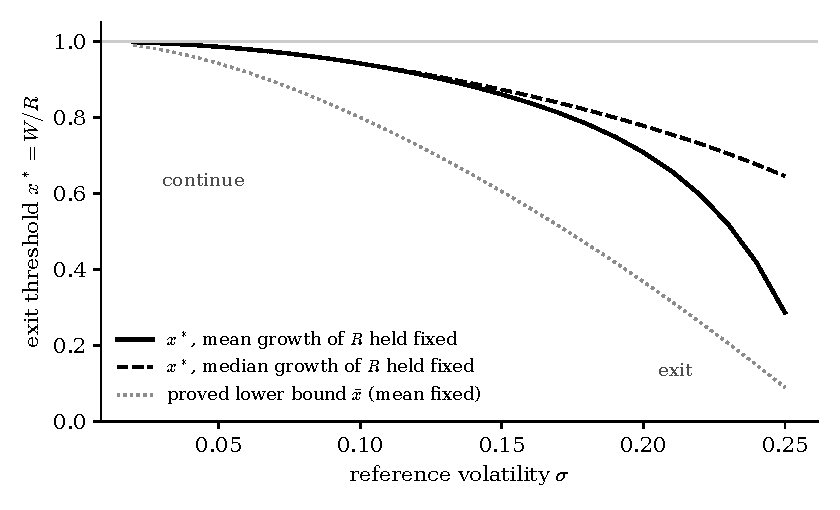
\includegraphics[width=0.82\textwidth]{fig1_volatility.pdf}
\caption{The quitting point falls as the benchmark becomes more volatile. Baseline calibration of Table~\ref{tab:calib}. The dotted line is the proved lower bound $\bar x$ of Theorem~\ref{thm:main}; the threshold always lies between it and par.}\label{fig:vol}
\end{figure}

The magnitude is large. With the drift gap fixed, doubling volatility from 10 to 20 percent widens the gap the agent will tolerate from 6 percent to 29 percent (Figure~\ref{fig:vol}). Under a mean-preserving spread the same doubling widens it from 6 to 18 percent. About half the first effect, then, comes from volatility's effect on the average path, and half from the spread itself.

\begin{proposition}[The bound falls with volatility]\label{prop:xbar}
Hold $\rho$ and $D<\rho$ fixed. Then $\bar x$ is strictly decreasing in $\sigma$, and $\bar x\to0$ as $\sigma\to\infty$. If $D<0$, then $\bar x\to1$ as $\sigma\to0$.
\end{proposition}

\begin{proof}
Appendix~\ref{app:B}.
\end{proof}

\noindent The limit $\sigma\to0$ with $D<0$ is the case in which the benchmark outruns wealth for sure. There the bound squeezes the threshold to par: with no chance that the gap closes by itself, there is nothing to wait for, and the agent quits as soon as she falls behind. These are Richter's unrescued rats.

\subsection{A benchmark that runs away, and loss aversion}

\begin{proposition}[Faster benchmarks and stronger loss aversion speed exit]\label{prop:drift}
Under Assumption~\ref{ass:main}, holding the other parameters fixed:
\begin{enumerate}[label=(\alph*)]
\item $x^*$ is nondecreasing in the drift gap $\delta$;
\item $x^*$ is strictly increasing in the loss-aversion parameter $\lambda$.
\end{enumerate}
\end{proposition}

\begin{proof}
Appendix~\ref{app:B}.
\end{proof}

\begin{inwords}
A benchmark that pulls away faster makes the agent quit sooner, and so does a shortfall that stings more.
\end{inwords}

Two parameters remain whose effects are numerical. A larger positional weight $\alpha$ lowers the threshold, and the effect grows with volatility: at $\sigma=0.05$ the threshold barely moves as $\alpha$ rises from $0.05$ to $3$, while at $\sigma=0.20$ it falls from $0.751$ to $0.592$. Caring more about standing scales up the pain of being behind, but it also scales up the reward for getting ahead and the value of the chance to get there, and in a volatile environment the second channel dominates. Greater impatience $\rho$ raises the threshold.

\begin{result}[Positional weight and impatience]\label{res:cs}
At the baseline, $x^*$ is decreasing in $\alpha$, with the effect increasing in $\sigma$, and increasing in $\rho$, as in Table~\ref{tab:cs}.
\end{result}

\begin{table}[t]
\centering\small
\caption{How the quitting point moves at the baseline ($\rho=0.05$, $\delta=0.02$, $\sigma=0.10$, $\alpha=0.5$, $\lambda=2$)}\label{tab:cs}
\begin{tabular}{@{}lllll@{}}
\toprule
Parameter & Range & $x^*$ moves from & Exit & Status \\
\midrule
Loss aversion $\lambda$ & $1\to4$ & $0.926\to0.956$ & sooner & proved \\
Drift gap $\delta$ & $0.005\to0.05$ & $0.926\to0.960$ & sooner & proved \\
Impatience $\rho$ & $0.04\to0.10$ & $0.932\to0.967$ & sooner & numerical \\
Positional weight $\alpha$, $\sigma=0.05$ & $0.05\to3$ & $0.986\to0.986$ & no change & numerical \\
Positional weight $\alpha$, $\sigma=0.10$ & $0.05\to3$ & $0.943\to0.935$ & later & numerical \\
Positional weight $\alpha$, $\sigma=0.20$ & $0.05\to3$ & $0.751\to0.592$ & later & numerical \\
\bottomrule
\end{tabular}
\end{table}

\subsection{Time left in the race}\label{sec:deadline}

Theorem~\ref{thm:main} gives the agent forever. That matters most where Proposition~\ref{prop:reduction} draws its line. When $\rho\le D$, her standing is expected to grow faster than she discounts the future, the race is worth infinitely much, and no shortfall is large enough to make her quit. Real races end. A first home has to be bought within a working life, and the comparison with peers fades at retirement. Suppose, then, that the race ends after $s$ more years: exit must come by then, and afterwards only consumption counts. Let $F_s$ be the value of staying, defined as $F$ in Proposition~\ref{prop:reduction} but with exit times no later than $s$.

\begin{proposition}[A deadline]\label{prop:deadline}
Let $\rho>0$, $\sigma>0$, $\alpha>0$ and $\lambda\ge1$; the condition $\rho>D$ is not needed. With $s>0$ years left in the race:
\begin{enumerate}[label=(\alph*)]
\item $V(W,R)=V_{\rm stop}(W)+F_s\big(\log(W/R)\big)$, and $0\le F_s(y)\le\alpha e^y\int_0^s e^{(D-\rho)t}\,dt$.
\item There is a threshold $x^*_s\in(0,1]$ such that immediate exit is optimal exactly when $x\le x^*_s$. For every $\rho'\ge\rho$ with $\rho'>D$, $x^*_s\ge e^{-(\rho'-\rho)s}\,\bar x(\rho')$, where $\bar x(\rho')$ is the bound $\bar x$ of Theorem~\ref{thm:main} computed with discount rate $\rho'$.
\item $x^*_s$ is nonincreasing in $s$: with more time left, she tolerates a wider gap.
\item As $s\to\infty$, $x^*_s$ decreases to the threshold $x^*$ of Theorem~\ref{thm:main} if $\rho>D$, and to $0$ if $\rho\le D$.
\end{enumerate}
\end{proposition}

\begin{proof}
Appendix~\ref{app:B}.
\end{proof}

\begin{inwords}
A deadline gives every race a quitting point. With little time left, a small shortfall is enough to make her stop, because there is little time for the gap to close. With more time left she holds on through a wider gap. Where Theorem~\ref{thm:main} applies, the quitting point settles at $x^*$ as the horizon lengthens. Where it does not, the quitting point keeps falling as the horizon lengthens, but every finite horizon has one. Of two people equally far behind, the one with less time left quits first.
\end{inwords}

Table~\ref{tab:deadline} puts numbers on it. At the baseline, time barely matters once five years remain: the quitting point is within 0.004 of $x^*$. With a more volatile benchmark the horizon matters more, because waiting for a swing takes time. The third row lies outside Theorem~\ref{thm:main}. Its benchmark is volatile enough ($\sigma=0.25$) that $D>\rho$, and with forever to wait the agent would never quit. With a working life she does: at 69 percent of the benchmark with ten years left, and at 50 percent with forty.

\begin{table}[t]
\centering\small
\caption{The quitting point $x^*_s$ by years left in the race ($\rho=0.05$)}\label{tab:deadline}
\begin{tabular}{@{}lcccccc@{}}
\toprule
 & \multicolumn{5}{c}{Years left, $s$} & No deadline \\
\cmidrule(lr){2-6}
 & 1 & 5 & 10 & 20 & 40 & $x^*$ \\
\midrule
Baseline & 0.966 & 0.946 & 0.944 & 0.942 & 0.942 & 0.942 \\
Moderate volatility & 0.932 & 0.878 & 0.852 & 0.835 & 0.823 & 0.818 \\
Volatile, $D>\rho$ & 0.882 & 0.763 & 0.689 & 0.604 & 0.503 & none \\
\bottomrule
\end{tabular}
\par\smallskip\parbox{0.92\textwidth}{\footnotesize Baseline and moderate volatility are the first two rows of Table~\ref{tab:calib}. The third row has $\sigma=0.25$, $\delta=0.01$, $\alpha=0.5$ and $\lambda=2$, so $D=0.0525>\rho$. Computed by backward induction on the variational inequality for $F_s$ (Appendix~\ref{app:C}). In the first two rows $\rho>D$ and $x^*_s$ approaches $x^*$; in the third $\rho<D$, there is no stationary threshold, and $x^*_s$ keeps falling (0.330 at $s=100$).}
\end{table}

The deadline also separates what the trend decides from what time decides. The sign of $\rho-D$, fixed by the benchmark's drift and volatility and by impatience, sets the floor that the quitting point approaches for those with the most time left: $x^*$ when $\rho>D$, and zero when $\rho\le D$. Standing and time left decide who reaches the quitting point first.

\section{The cost of keeping someone in the race}\label{sec:welfare}

\subsection{The exact cost}\label{sec:exact}

Suppose an intervention keeps the agent in the race past her threshold. It might be a commitment device, a default, a counselor's encouragement, or a program that conditions support on continued pursuit of the benchmark. Model it as an exit time $\tilde\tau$ imposed on the agent, who still chooses consumption. Write $J(y;q,\tilde\tau)$ for the expected payoff inside $F$ in Proposition~\ref{prop:reduction} under consumption shares $q$ and exit time $\tilde\tau$, so her welfare is $V_{\rm stop}(W)+J(y;q,\tilde\tau)$, and write $b:=\log x^*$ for the threshold in log terms.

The cost has an exact expression in terms of a flow shortfall $\Delta$. Above the threshold ($y>b$), let
\[
\Delta(y,q):=qF'(y)+H_\rho(q)-\log\big(1+\rho F'(y)\big)\ \ge0,
\]
the utility lost by consuming the share $q$ instead of the optimal share $q^*(y)$; it is zero exactly at $q=q^*(y)$. At or below the threshold ($y\le b$), let
\[
\Delta(y,q):=H_\rho(q)-f(y)\ \ge\ \alpha\lambda\,(1-e^{y})>0,
\]
the flow the agent gives up by being in the race at all when she would rather be out. The bound $\alpha\lambda(1-x)$ is the loss-weighted sting of her shortfall.

\begin{proposition}[The welfare cost of an imposed exit rule]\label{prop:welfare}
Under Assumption~\ref{ass:main}, let $q$ be a bounded consumption share and $\tilde\tau$ any exit time. Then
\[
F(y)-J(y;q,\tilde\tau)\;=\;\E_y\int_0^{\tilde\tau}e^{-\rho t}\,\Delta(y_t,q_t)\,dt\;+\;\E_y\big[e^{-\rho\tilde\tau}F(y_{\tilde\tau});\ \tilde\tau<\infty\big].
\]
\end{proposition}

\begin{proof}
Appendix~\ref{app:B}.
\end{proof}

\begin{inwords}
The cost of an imposed exit rule has three parts. Every moment spent in the race below her threshold costs the agent the full sting of her shortfall. Time above the threshold costs nothing if she consumes optimally. And if the rule pushes her out while staying still had value, she loses that value.
\end{inwords}

The decomposition makes the sign of the loss transparent for threshold rules, the natural form of an intervention that says ``keep going until you fall to $\tilde x$'' or ``stop once you fall to $\tilde x$.''

\begin{corollary}\label{cor:welfare}
Let $\tilde\tau$ be the first time $x_t\le\tilde x$, with consumption bounded and $x_0>\tilde x$.
\begin{enumerate}[label=(\alph*)]
\item If $\tilde x<x^*$ (forced continuation), the loss is at least $\alpha\lambda\,\E\int_0^{\tilde\tau}e^{-\rho t}(1-x_t)\mathbf 1_{\{x_t\le x^*\}}dt>0$.
\item If $\tilde x>x^*$ (forced early exit), the loss is at least $F(\log\tilde x)\,\E[e^{-\rho\tilde\tau}]>0$.
\end{enumerate}
\end{corollary}

\begin{proof}
Both bounds drop nonnegative terms from Proposition~\ref{prop:welfare}. In (a) the ratio must pass through $(\tilde x,x^*]$ before $\tilde\tau$, and with $\sigma>0$ and bounded consumption it does so with positive probability, spending positive time there. In (b), $F>0$ above $\log x^*$ by Theorem~\ref{thm:main}, and $\tilde\tau<\infty$ with positive probability.
\end{proof}

How large is the loss? Let the agent choose consumption optimally given the imposed rule; this can include consuming faster than $\rho W$ to reach the imposed exit sooner. Figure~\ref{fig:welfare} plots the loss at par against the imposed threshold.

\begin{result}[Quadratic loss]\label{res:quad}
At the baseline, the loss at par is $c\,(\log\tilde x-\log x^*)^2$ with $c$ between 5.37 and 5.56 for every imposed threshold computed, from $\tilde x=0.80$ to $\tilde x=0.97$. In the high-volatility calibration the same ratio lies between 14 and 23 over $\tilde x\in[0.50,0.75]$: the loss is quadratic near the threshold and grows somewhat more slowly than that for large forced continuations.
\end{result}

\begin{figure}[t]
\centering
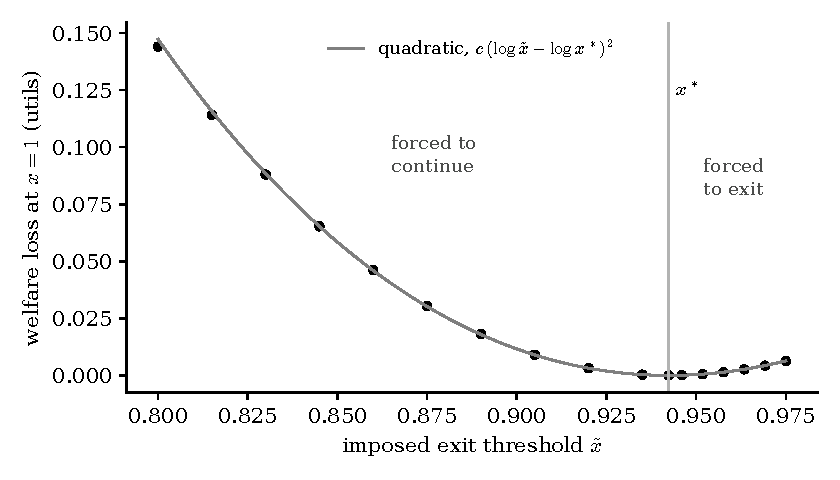
\includegraphics[width=0.82\textwidth]{fig2_welfare.pdf}
\caption{Welfare loss at par from an imposed quitting point $\tilde x$, baseline calibration. The agent chooses consumption optimally given the imposed rule. The loss is zero at $x^*$ and rises quadratically on both sides.}\label{fig:welfare}
\end{figure}

The quadratic shape has a consequence for how interventions should be judged. A small push past the threshold costs almost nothing, because the first-order effect vanishes at an optimum. Each further push costs more than the one before. At the baseline, keeping the agent in until $x=0.90$ instead of $0.942$ costs 63 percent of what the race was worth to her at par, and keeping her in until $0.85$ costs 315 percent: she would have been better off quitting on the spot. In consumption units these numbers are small at the baseline, where the whole race is worth as much as a permanent 0.09 percent rise in consumption, and forcing her to $0.85$ hurts as much as a permanent 0.29 percent cut. They are not small in the high-volatility calibration, where the race is worth as much as a permanent 31 percent rise and forcing continuation from $0.663$ to $0.50$ hurts as much as a permanent 5.5 percent cut (Appendix~\ref{app:C} gives the conversion).

\paragraph{Who should be nudged?} Proposition~\ref{prop:welfare} turns the policy question into a diagnostic one. A patience intervention helps an agent who would quit above her threshold, which is what a doer's lapse looks like, and harms one who quits at it. Allcott and Taubinsky (2015) and Bernheim and Rangel (2009) show that a nudge's welfare effect depends on the share of biased agents it reaches. The present model adds that the unbiased share may be larger than it looks: it includes agents whose disengagement is the correct response to a benchmark that has moved away from them. Telling the two groups apart requires knowing where an agent stands relative to her threshold, and by Theorem~\ref{thm:vol} that depends on how volatile her benchmark is.

\paragraph{A normative caveat.} The welfare results evaluate interventions by the agent's own preferences, loss aversion included. A planner who regards loss aversion itself as a bias would use a different welfare function and could reach different conclusions. That view would be a reason to change the agent's preferences, not a reason to keep her in a race that her preferences, as they are, tell her to leave.

\subsection{What ``worse off'' means}\label{sec:worse}

In the model, being held below her threshold costs the agent the full, loss-weighted sting of her shortfall every period. The evidence on people who cannot let go of unreachable goals shows what that looks like in a life.
\begin{itemize}
\item Adults who disengage less readily from unattainable goals report more depressive symptoms, more stress and more physical health problems, and show less normative daily cortisol rhythms (Wrosch, Miller, Scheier and Brun de Pontet 2007).
\item Adolescents who had the most trouble letting go showed systemic inflammation rising about twice as fast as average over a year, independent of depression, weight and smoking. The authors conclude that ``in some contexts, persistence may actually undermine wellbeing and good health'' (Miller and Wrosch 2007).
\item Low mood may exist partly to foster ``disengagement from commitments to unreachable goals'' (Nesse 2000). Pushing someone past the point where her mood is telling her to stop overrides the signal that would end the episode.
\item The World Health Organization (2019) defines burn-out by exhaustion, ``increased mental distance from one's job'' and reduced efficacy. Joint WHO and ILO estimates attribute 745,194 deaths from heart disease and stroke in 2016 to working 55 or more hours a week (Pega et al.\ 2021).
\end{itemize}
These studies are observational. They measure people's own capacity to let go rather than outside pressure to hold on, but outside pressure is exactly what makes letting go harder. ``Mental distance from one's job'' is also what quiet quitting looks like from outside, so observed disengagement can be an agent optimally waiting near her threshold or one already pushed too far. Either way the model's answer is the same: do not push harder. Two limits apply. The model counts only the cost incurred while she is held in the race, and the physiological findings suggest that the damage outlasts it, so the losses of Section~\ref{sec:exact} are lower bounds. And exit here means letting go of a comparison, not leaving a job, school, treatment or relationship; what the model warns against is pressure to keep measuring oneself against a target that has moved out of reach.

\subsection{From one agent to an economy}\label{sec:aggregate}

The model describes one person, but its benchmark is shared: everyone saving for a house in the same market faces the same price. A shock to the benchmark moves a whole cohort's standing at once, so the share of the cohort at or below its threshold, and the grind of those still in the race, are functions of the benchmark's path.

\paragraph{An illustration.} Table~\ref{tab:cohort} spreads the baseline agent's standing across a cohort, with log standing normally distributed around par with standard deviation 0.25. It asks two things of each scenario: the share of the cohort at or below its threshold, and the cohort's sacrifice for the race, measured as the average shortfall of consumption below what each member would consume out of the race, with zero for those already out. The levels depend on the assumed spread and mean little; the changes are the point. A one-time 10 percent jump in the benchmark, the announced finish line suddenly extended, raises the share out of the race from 41 to 56 percent and cuts the cohort's grind by more than a third. A benchmark twice as volatile has the opposite effect from a faster one: it keeps most of the cohort in the race, and those in it grind harder, because the chance that the gap closes is worth more. The companion tool (see Data and code) lets a reader change every input, including the spread of the cohort and its preferences.

\begin{table}[t]
\centering\small
\caption{An illustrative cohort (baseline preferences; log standing $\sim N(0,0.25^2)$ across the cohort)}\label{tab:cohort}
\begin{tabular}{@{}lccc@{}}
\toprule
Scenario & $x^*$ & Share out of the race & Average grind \\
\midrule
Baseline (drift gap 2 pts, volatility 10\%) & 0.942 & 41\% & 5.2\% \\
Benchmark runs 2 points a year faster & 0.956 & 43\% & 3.8\% \\
Benchmark jumps 10\% once & 0.942 & 56\% & 3.3\% \\
Benchmark twice as volatile & 0.708 & 8\% & 19.1\% \\
Drift gap narrowed to 1 point & 0.932 & 39\% & 6.3\% \\
\bottomrule
\end{tabular}
\par\smallskip\parbox{0.92\textwidth}{\footnotesize Average grind is the cohort mean of $(\rho-q^*)/\rho$, the proportional shortfall of consumption below its post-exit level, with zero for members at or below the threshold. Computed with the solver of Appendix~\ref{app:C}.}
\end{table}

\paragraph{The aggregate now.} Several national series move the way the model says a runaway benchmark would move them. None was designed to measure the model's mechanism, each has other causes, and the model does not claim to explain them. They show what is at stake if the mechanism is at work, and how the effects compound.
\begin{itemize}
\item \emph{First order: effort and output.} The fall in engagement and its estimated cost, about 1.9 trillion dollars a year in the United States (Section~\ref{sec:intro}), are the first-order effect. In the model, disengagement is the grind falling toward zero, and the grind is the sacrifice, in saving or effort, that the race was drawing out.
\item \emph{Second order: despair and the diseases that follow it.} The share of U.S. adults who currently have or are being treated for depression rose from about 10 percent in 2015 to 18.3 percent in 2025; among adults under 30 it doubled, from 13.0 percent in 2017 to 26.7 percent (Witters 2025). Alcohol and drug misuse cost the United States more than 442 billion dollars a year in health care, criminal justice and lost productivity (Murthy 2016). The share of U.S. adults in extreme distress rose from 3.6 percent in 1993 to 6.4 percent in 2019 (Blanchflower and Oswald 2020). In 2025 the United States fell to 24th in the World Happiness Report, its lowest position, on declining well-being among people under 30 (Helliwell et al.\ 2025). Depression and anxiety cost an estimated 12 billion working days a year worldwide (World Health Organization 2022). Section~\ref{sec:worse} describes the evidence linking prolonged pursuit of unattainable goals to outcomes of this kind.
\item \emph{Third order: household formation and expectations.} First-time buyers have fallen to a record-low 21 percent of home purchases (National Association of Realtors 2025). About three-quarters of American adults expect today's children to be worse off financially than their parents (Pew Research Center 2025). Each feeds the next round. A later first home is a later start on home equity, and a generation that expects to fall behind its parents has less reason to sacrifice for a race it does not expect to finish.
\end{itemize}

\paragraph{Hope as an aggregate.} In the model, hope is exact: it is the value of staying in the race, positive because the gap may still close. Summed over a cohort, it is collective hope, and a runaway benchmark is what destroys it. What brings a disengaged cohort back is what brought Richter's rats back: a real chance of catching up, from a benchmark that slows or resources that grow, not pressure on people for whom the race has stopped paying. The model takes wages and prices as given (it is partial equilibrium), so it cannot say how disengagement feeds back into them. But it links an observable benchmark to the share of a cohort that has stopped keeping score, which is what a policymaker needs to monitor.

A companion planning tool, The Hope Gap, runs this calculation with current public data for the nation, every state and county, and large cities (see Data and code).

\section{Risky wealth}\label{sec:wealth}

The baseline puts all the risk in the benchmark. Suppose instead that wealth is risky too:
\[
dW_t=(r_WW_t-c_t)\,dt+\sigma_WW_t\,dZ^W_t,\qquad dR_t=r_RR_t\,dt+\sigma_RR_t\,dZ^R_t,
\]
where $\sigma_W$ and $\sigma_R$ are the volatilities of wealth and of the benchmark, and the two Brownian motions have correlation $\varrho$. Let
\[
S:=\sigma_W^2+\sigma_R^2-2\varrho\,\sigma_W\sigma_R
\]
be the variance of the ratio's log per unit time, and assume $S>0$.

\begin{proposition}[Only the ratio's risk matters]\label{prop:wealth}
The value function is
\[
V(W,R)=\frac1\rho\log W+K_0-\frac{\sigma_W^2}{2\rho^2}+F_S\big(\log(W/R)\big),
\]
where $F_S$ is the function $F$ of Proposition~\ref{prop:reduction} computed with $\sigma^2$ replaced by $S$ and the median growth of the ratio $\mut$ replaced by $\mut_S:=r_W-r_R-\tfrac12\sigma_W^2+\tfrac12\sigma_R^2$. The value is finite if and only if $\rho>D_S:=\mut_S+\tfrac12S$. All conclusions of Theorem~\ref{thm:main} hold with these substitutions, and so do those of Theorem~\ref{thm:vol} for changes in $S$ that hold fixed $D_S$, $\mut_S$, or the effective drift gap $\delta_S:=\tfrac12S-\mut_S$. In particular the exit threshold depends on $(\sigma_W,\sigma_R,\varrho)$ only through $S$ and $\mut_S$.
\end{proposition}

\begin{proof}
Appendix~\ref{app:B}.
\end{proof}

\begin{inwords}
What matters for quitting is how much the agent's standing moves, not which side of the comparison does the moving. Risk in the benchmark and risk in her own wealth enter through one number, the variance of the ratio.
\end{inwords}

Proposition~\ref{prop:wealth} answers the question of why wealth is deterministic in the baseline: nothing is lost by making it so, because any economy with risky wealth is equivalent, for the exit decision, to one with deterministic wealth, benchmark volatility $\sqrt S$ and the same growth rates of the ratio. The baseline's $\sigma$ should be read as the volatility of the agent's standing.

The extension also sharpens the empirical content, with one caution. The effective drift gap $\delta_S=\delta+\sigma_W^2-\varrho\sigma_W\sigma_R$ differs from the raw gap $\delta$, so a comparison that holds $\delta$ fixed while wealth becomes riskier is not covered, and it can reverse (Appendix~\ref{app:C}). Two comparisons are covered. With independent income risk ($\varrho=0$), raising $\sigma_W$ raises $S$ and leaves $D_S$ unchanged, a mean-preserving spread of the ratio, so it delays exit. Raising the correlation $\varrho$ lowers $S$ and leaves $\mut_S$ unchanged, so it speeds exit. Both hold under the conditions of Theorem~\ref{thm:vol}. A household whose wealth is mostly home equity in the market whose prices it watches is the leading case of high correlation. Its standing barely moves when prices do, so, other things equal, it has less reason to wait than a renter saving toward a down payment in the same market, who faces the full volatility of local prices.

\section{Discussion}\label{sec:discussion}

\paragraph{Young workers, revisited.} The model's agent near her threshold is the closest formal counterpart of ``quiet quitting'': still in the race, barely sacrificing for it, staying for the chance that the benchmark comes back. For young workers, the distinction drawn in Section~\ref{sec:why} between a benchmark that runs away and one that wobbles is the important one. House prices that outrun incomes and entry-level jobs that pay less or disappear are drift gaps and push people to their thresholds; uncertainty about AI or housing, taken alone, keeps them in the race longer. Policies that steady a benchmark therefore cut both ways: slowing its growth keeps people in the race, while damping its swings pushes those near the threshold out sooner. The grind returns when standing improves, which requires the benchmark to stop running away. Proposition~\ref{prop:deadline} adds a caution about reading age differences. At the same standing, a worker with more of her working life ahead should tolerate a larger shortfall, not a smaller one. If young workers disengage first, the model says they are further behind, or face a benchmark pulling away faster, not that they give up more easily. None of this shows that any particular young worker is right, but it does show that the spread of such behavior cannot by itself be read as a loss of grit, and that an employer or policymaker who wants to change it should look at the benchmark before looking at the worker.

\paragraph{Exit, pauses and slowing down.} The model's exit is a permanent decision to stop scoring oneself against the benchmark, and it is not free. After exit the agent consumes the share $\rho$ of her wealth, and when, as at the baseline, $\rho$ exceeds the return on wealth, her wealth shrinks while the benchmark keeps growing. Someone who stops comparing herself with the local price of a house does not quietly save her way back to it; the house moves out of reach, and coming back to the race would mean coming back much further behind. Temporary withdrawal with the option to return would be a switching problem with re-entry, of which the irreversible case is the limit in which re-entry is prohibitively costly. Costly re-entry should raise the threshold, since exit would then destroy less; that case is not analyzed here.

\paragraph{Empirical tests.} The model makes three predictions that do not follow from accounts without a stochastic benchmark. First, holding the drift of a benchmark fixed, people facing more volatile benchmarks should persist longer in losing comparisons. Second, the effect of how much a person cares about standing on persistence should be larger where benchmarks are more volatile. Third, co-movement between a person's resources and her benchmark should shorten persistence. Each can be tested where benchmark volatility varies across markets or cohorts, for example local house-price volatility across metropolitan areas, combined with survey measures of aspirations and hours. A real-effort experiment in which subjects chase a target that is either steady or volatile, with the same expected path, would test the first prediction directly.

\paragraph{What is proved and what is computed.} Everything labeled Theorem, Proposition or Corollary is proved; Results~\ref{res:vol} to \ref{res:quad} rest on the collocation solver of Appendix~\ref{app:C}, which reproduces every proved property of Theorem~\ref{thm:main} in all cases checked. Closing the gap in Theorem~\ref{thm:vol} requires controlling the concavity that loss aversion introduces near par. No condition on the primitives that implies convexity is known; the 19 computed cases in which it fails all have $\alpha\ge1$ and $\lambda\ge2$.

\paragraph{Limits.} Log utility delivers the one-dimensional reduction; with other power utilities the problem is two-dimensional and the results are not established here. The preferences have no probability weighting; adding it reintroduces the never-stopping problem of Ebert and Strack (2015). The positional payoff is piecewise linear in the ratio; curvature in the gain and loss domains would change magnitudes.

\section{Conclusion}\label{sec:conclusion}

When the target moves at random, giving up on it can be the plan rather than a lapse. That is what the paper proves: it locates the quitting point, shows which way volatility moves it, and writes down the cost of overriding it. The finding matters most at scale. The benchmarks that define getting ahead in the United States, a first home and a fair share of the growth one helps produce, have been pulling away from the pay that chases them for four decades. The model says what that does: it moves whole cohorts toward the point where the race stops paying, and then past it. What follows looks like a loss of grit, and it is expensive: disengaged workers, deferred households, and the strain on health and life that the evidence attaches to being held in a losing race. But the model also locates the cause, and the remedy, in the benchmark rather than the worker. Pushing harder on people who have stopped keeping score adds to the cost. Restoring a real chance of catching up, by slowing the benchmarks that have run away or raising the resources that chase them, is what brings them back.

That remedy can now be measured. The quantities the model needs, the drift and volatility of a benchmark and where a group stands against it, are published monthly or quarterly for the nation and the states. Federal, state, county and city officials can compute, for the people they serve, how many have stopped keeping score, how many are near the edge, and how far a benchmark must slow to bring them back. They can track that number the way they track unemployment. The companion tool does this with current data. A society that waits for disengagement to show up in output, health and household formation has waited too long.

\section*{Acknowledgment}
I thank Richard Thaler for putting me in touch with Hersh Shefrin, and Hersh Shefrin for generous guidance that reshaped this revision, including the evidence on moving focal points. I thank Debraj Ray for a correction on the history of the aspirations literature. None of them has reviewed the full paper, and errors are mine.

This paper was developed with extensive use of AI systems. Anthropic's Claude was used for derivations, numerical code and drafting. The proofs in Appendices~\ref{app:A} and \ref{app:B} were tested through repeated rounds of adversarial review by OpenAI's ChatGPT and DeepSeek, each asked to find errors in the full text; every claimed error was checked, and those confirmed were corrected. The author takes full responsibility for the content.

\section*{Data and code}
All numerical results, both figures and every table are produced by the Python code in the replication package, Lester (2026), at \url{https://doi.org/10.7910/DVN/V5NSZX}.

The interactive companion, The Hope Gap (\url{https://lesterhau.github.io/rational-foreclosure/}), refreshes itself twice a week with public data on prices, pay, home values and population for the nation, every state and county, and large cities. An official chooses a place, a benchmark (owning a home, or keeping up with the cost of living) and a group. The tool identifies the growth of the agent's resources net of post-exit consumption, $r_W-\rho$, with the growth of pay, so the finiteness line $\rho=D$ of Proposition~\ref{prop:reduction} becomes: benchmark growth minus pay growth equals $\sigma^2$. It reports how far an area sits from that line (its Hope Gap), where the quitting point falls, how many people are past it, how that changes over two years under several scenarios, and what it would take in homes built or pay growth to close the gap, with a dated plan for that office. By default the race ends at age 67, as in Proposition~\ref{prop:deadline}, so each person's quitting point depends on the working years left; the user can remove the deadline. Each group's pay trend is the area's adjusted by how that group's earnings have grown relative to all workers (Census Bureau, Quarterly Workforce Indicators), and the lowest income group is measured against starter homes, so groups can be compared side by side. One departure from the model is labeled as such: by default, people take about a year to notice a change in the trend, and the user can make it immediate, as in the model. The paper's two figures can be reproduced and varied there as well.

\clearpage
\appendix
\section{Proofs of Proposition~\ref{prop:reduction} and Theorem~\ref{thm:main}}\label{app:A}

This appendix is self-contained. It uses only standard tools: It\^o's formula for $C^2$ functions, optional stopping at bounded stopping times, the law of large numbers $Z_t/t\to0$, existence, uniqueness and continuous dependence for ordinary and stochastic differential equations with locally Lipschitz coefficients, Gr\"onwall's inequality, Dini's theorem, and the convergence theorems of integration. The dynamic programming step, the comparison step and a generalized It\^o formula, which standard treatments cite, are proved here. Where a published theorem covers the same ground it is named, and it was checked against the source. Proposition~\ref{prop:reduction} is Lemmas~\ref{lem:reduction} and \ref{lem:finite}; Theorem~\ref{thm:main} collects Lemmas~\ref{lem:mono}, \ref{lem:above}, \ref{lem:below}, \ref{lem:reg}, \ref{lem:sf}, \ref{lem:kink}, Theorem~\ref{thm:threshold} and Theorem~\ref{thm:verif}.


\subsection{Setting}

Wealth evolves as $dW_t=(r_W W_t-c_t)\,dt$ and the reference as $dR_t=r_R R_t\,dt+\sigma R_t\,dZ_t$ with $\sigma>0$. Write consumption as a fraction of wealth, $c_t=q_tW_t$, and work with the log ratio $Y_t=\log(W_t/R_t)$. By It\^o's formula,
\begin{equation}
dY_t=(\mut-q_t)\,dt-\sigma\,dZ_t,\qquad \mut:=r_W-r_R+\tfrac12\sigma^2 . \label{eq:Y}
\end{equation}
Set
\begin{equation}
D:=\mut+\tfrac12\sigma^2=r_W-r_R+\sigma^2,\qquad f(y):=\alpha\,v(e^y-1),\qquad H_\rho(q):=\frac q\rho-1-\log\frac q\rho\ \ (\ge 0),
\end{equation}
where $v(u)=u$ for $u\ge0$ and $v(u)=\lambda u$ for $u<0$, with $\alpha>0$ and $\lambda\ge1$. Note that $E[e^{Y_t}]\le e^{y+Dt}$ for every control with $q\ge0$, since consumption only lowers $Y$ pathwise.

\begin{adefinition}[Plans and strategies]\label{def:plans}
A \emph{consumption rate} is a progressively measurable process $q\ge0$ with $\int_0^t q_s\,ds<\infty$ a.s.\ for all $t$; consumption is $c_t=q_tW_t$ for all $t\ge0$, before and after exit. A \emph{plan} is a consumption rate together with an exit time $\tau\in[0,\infty]$, a stopping time. Writing
\[
P_T:=\int_0^T e^{-\rho t}\big[\log c_t+\mathbf 1_{\{t<\tau\}}f(Y_t)\big]\,dt,
\]
the value of a plan is $\limsup_{T\to\infty}E[P_T]$, and $V(W,R)$ is the supremum of the value over \emph{all} plans. No admissibility restriction is imposed: no transversality condition, no integrability condition on consumption beyond $\int_0^tq_s\,ds<\infty$. Each $E[P_T]$ is well defined in $[-\infty,\infty)$, because $E[P_T^+]<\infty$ when $\rho>D$, by Lemma~\ref{lem:burst} and the budget identity \eqref{eq:budget} below (a pathwise identity whose derivation does not use this fact), and $\limsup$ is the most permissive way to aggregate the truncations: any plan whose truncated payoffs converge gets its limit, and no plan is helped by the choice. For the reduced problem, a \emph{strategy} is the pair $(q,\tau)$ restricted to $[0,\tau)$. A \emph{reference system} is a filtered probability space satisfying the usual conditions, carrying a Brownian motion $Z$ whose increments after each time $t$ are independent of $\cF_t$ (hence, by optional sampling, after each bounded stopping time as well). Strategies and plans live on an arbitrary reference system, and every supremum over them, $V$, $F$ and later $F_\varepsilon$, also runs over the system. The generality costs nothing: every upper bound below is proved strategy by strategy on an arbitrary system, and the supremum is attained by a feedback control on the plain Brownian filtration (Theorem~\ref{thm:verif}). It earns its keep exactly once, in Lemma~\ref{lem:cond}, where conditioning on a past event produces a system whose initial $\sigma$-field is rich. Let $\cA$ denote the set of consumption rates and $\cT$ the set of stopping times. Payoffs take values in $[-\infty,\infty]$, with $H_\rho(0):=+\infty$ and $\log0:=-\infty$.
\end{adefinition}

\begin{aremark}[The choice of convention is harmless]\label{rem:conv}
An improper expected payoff whose integrand is unbounded in both signs needs a convention, whatever the model. The one above is explicit, and nothing in the results depends on it: whenever a plan's truncated payoffs $E[P_T]$ converge, the $\limsup$ is that limit, so the two agree on every plan for which the original improper expectation is unambiguous; the optimal plan of Theorem~\ref{thm:verif} is of this kind. For any other convention that agrees with the ordinary expectation in the unambiguous cases and never exceeds $\limsup_TE[P_T]$ in the remaining ones, the supremum over plans is the same number, since the upper bound of Lemma~\ref{lem:reduction} caps every plan and the optimum attains it with an honest limit.
\end{aremark}

The \emph{continuation advantage} is
\begin{equation}
F(y):=\sup_{q\in\cA,\ \tau\in\cT} J(y;q,\tau),\qquad J(y;q,\tau):=E_y\!\int_0^\tau e^{-\rho t}\big[f(Y_t)-H_\rho(q_t)\big]\,dt . \label{eq:F}
\end{equation}

\begin{alemma}[Consumption above $\rho W$ never helps]\label{lem:trunc}
For any strategy $(q,\tau)$, the pair $(q\wedge\rho,\tau)$ is a strategy and $J(y;q\wedge\rho,\tau)\ge J(y;q,\tau)$. Hence the supremum in \eqref{eq:F} may be taken over controls with values in $[0,\rho]$, and every strategy used below has this property. Moreover, if $q\le\rho$, then $e^{-\rho T}|\log W_T|\to0$ deterministically.
\end{alemma}

\begin{proof}
Since $q\wedge\rho\le q$, \eqref{eq:Y} gives $Y^{q\wedge\rho}_t\ge Y^q_t$ pathwise, so $f(Y^{q\wedge\rho}_t)\ge f(Y^q_t)$ because $f$ is nondecreasing. Also $H_\rho(q_t\wedge\rho)\le H_\rho(q_t)$: the two coincide where $q_t\le\rho$, and where $q_t>\rho$ the left side is $H_\rho(\rho)=0$. Integrating the difference of the two integrands, which is nonnegative, up to the same $\tau$ gives $J(y;q\wedge\rho,\tau)\ge J(y;q,\tau)$. For the last claim: if $q\le\rho$, then $\log W_0+(r_W-\rho)t\le\log W_t\le\log W_0+r_Wt$, so $e^{-\rho T}|\log W_T|\to0$ deterministically.
\end{proof}

\begin{alemma}[Late consumption bursts have no value]\label{lem:burst}
For every $q\ge0$ and $0\le s<T$,
\begin{equation}
\frac{e^{-\rho T}}{\rho}\,q\ \le\ e^{-\rho s}H_\rho(q)\ -\ e^{-\rho s}\log\!\big(1-e^{-\rho(T-s)}\big). \label{eq:legendre}
\end{equation}
Consequently, for every consumption rate, pathwise, with $Q(t):=\int_0^t q_s\,ds$ and every $0\le t_0\le T$,
\begin{equation}
\frac{e^{-\rho T}}{\rho}\big(Q(T)-Q(t_0)\big)\ \le\ \int_{t_0}^T e^{-\rho s}H_\rho(q_s)\,ds\ +\ e^{-\rho t_0}g(T-t_0), \label{eq:burst}
\end{equation}
where $g(u):=\int_0^u -e^{-\rho r}\log(1-e^{-\rho(u-r)})\,dr$ satisfies $0\le g(u)\le e^{-\rho u}\big[\frac{u}{1-e^{-\rho}}+e^{\rho}c_\rho\big]\to0$ as $u\to\infty$, with $c_\rho:=\int_0^1-\log(1-e^{-\rho v})\,dv<\infty$.
\end{alemma}

\begin{proof}
Fix $s<T$ and set $\theta:=e^{-\rho(T-s)}\in(0,1)$. The map $q\mapsto(e^{-\rho T}/\rho)q-e^{-\rho s}H_\rho(q)$ is concave, tends to $-\infty$ at $q\downarrow0$ and as $q\to\infty$, and its stationary point is $q^*=\rho/(1-\theta)$. There its value is
\[
e^{-\rho s}\Big[\frac{\theta}{1-\theta}-H_\rho\Big(\frac{\rho}{1-\theta}\Big)\Big]
=e^{-\rho s}\Big[\frac{\theta}{1-\theta}-\frac{\theta}{1-\theta}-\log(1-\theta)\Big]=-e^{-\rho s}\log(1-\theta),
\]
which is \eqref{eq:legendre}. Integrating \eqref{eq:legendre} over $s\in[t_0,T)$ along any measurable path $s\mapsto q_s$ gives \eqref{eq:burst}, after the substitution $r=s-t_0$ in the error term. For the bound on $g$, substitute $v=u-r$, so $g(u)=e^{-\rho u}\int_0^u e^{\rho v}\big[-\log(1-e^{-\rho v})\big]dv$. If $u\le1$, this is at most $e^{-\rho u}e^{\rho}c_\rho$. If $u>1$, split at $r=u-1$: on $[0,u-1]$, $-\log(1-x)\le x/(1-x)$ gives $-\log(1-e^{-\rho(u-r)})\le e^{-\rho(u-r)}/(1-e^{-\rho})$, so that piece is at most $ue^{-\rho u}/(1-e^{-\rho})$; on $(u-1,u]$, bound $e^{-\rho r}\le e^{-\rho(u-1)}$ and substitute $v=u-r$ to get $e^{\rho}e^{-\rho u}c_\rho$, where $c_\rho$ is finite because the singularity of $-\log(1-e^{-\rho v})\sim\log\frac1{\rho v}$ at $v=0$ is integrable.
\end{proof}

The name is exact: in the finite-horizon budget identity below, the only way a plan can beat $V_{\rm stop}$ is through the term $e^{-\rho T}Q(T)/\rho$, which is large only if consumption explodes near the horizon; \eqref{eq:burst} says the consumption cost of such a burst cancels the gain, up to an error that vanishes with the horizon. This is what makes any transversality assumption unnecessary.

\begin{alemma}[Reduction]\label{lem:reduction}
Let $V_{\rm stop}(W)=\frac1\rho\log W+K_0$ with $K_0=\frac{\log\rho}{\rho}+\frac{r_W-\rho}{\rho^2}$, the value of log consumption after exit, and let $\rho>D$. Then for all $W,R>0$,
\[
V(W,R)=V_{\rm stop}(W)+F\big(\log(W/R)\big),
\]
with the supremum over all plans: $\limsup_{T\to\infty}E[P_T]\le V_{\rm stop}(W)+F(\log(W/R))$ for every plan, and the bound is attained, as an honest limit, by the optimal plan of Theorem~\ref{thm:verif} extended by $q\equiv\rho$ after exit. If $\rho\le D$, both sides are $+\infty$.
\end{alemma}

\begin{proof}
Let $\ell_t=\log W_t$, so $d\ell_t=(r_W-q_t)\,dt$ and $\ell_T=\ell_0+r_WT-Q(T)$. Fix a plan and a deterministic horizon $T$. The product rule gives, pathwise,
\[
e^{-\rho T}\frac{\ell_T}{\rho}-\frac{\ell_0}{\rho}=\int_0^T e^{-\rho t}\Big[\frac{r_W-q_t}{\rho}-\ell_t\Big]dt,
\qquad
e^{-\rho T}K_0-K_0=-\rho K_0\int_0^T e^{-\rho t}dt .
\]
Adding, and using $\log c_t=\log q_t+\ell_t$ and $\rho K_0=\log\rho+r_W/\rho-1$,
\begin{equation}
\int_0^T e^{-\rho t}\log c_t\,dt
=V_{\rm stop}(W_0)+d(T)+\frac{e^{-\rho T}}{\rho}Q(T)-\int_0^T e^{-\rho t}H_\rho(q_t)\,dt, \label{eq:budget}
\end{equation}
where $d(T):=-e^{-\rho T}[(\ell_0+r_WT)/\rho+K_0]$ is deterministic and $d(T)\to0$. The identity is ordinary calculus along each path; if $\int_0^T(\log q_t)^-\,dt=\infty$ on a path, both sides are $-\infty$ there and every inequality below holds trivially. (The positive part is harmless: $(\log q)^+\le q$ and $Q(T)<\infty$.)

\emph{Upper bound, all plans.} Fix $t_0\in(0,T)$ and set $w:=1-e^{-\rho(T-t_0)}\in(0,1)$. Apply \eqref{eq:burst} twice: on $[t_0,T]$ as stated, and on $[0,t_0]$ at horizon $t_0$, multiplied by $e^{-\rho(T-t_0)}$. Together,
\[
\frac{e^{-\rho T}}{\rho}Q(T)-\int_0^T e^{-\rho t}H_\rho\,dt\ \le\ e^{-\rho(T-t_0)}g(t_0)+e^{-\rho t_0}g(T-t_0)\ -\ w\int_0^{t_0}e^{-\rho t}H_\rho\,dt .
\]
Add the positional term. Pathwise $Y_t\le Y^0_t$, the uncontrolled ratio, and $f^+(y)\le\alpha e^y$ with $E[e^{Y^0_t}]=e^{y+Dt}$, so
\[
E\int_0^{T\wedge\tau}e^{-\rho t}f(Y_t)\,dt\ \le\ E\int_0^{t_0\wedge\tau}e^{-\rho t}f(Y_t)\,dt\ +\ \frac{\alpha e^{y}e^{-(\rho-D)t_0}}{\rho-D}.
\]
Dropping the cost on $(t_0\wedge\tau,t_0]$ and scaling by $w$,
\[
E\Big[\int_0^{t_0\wedge\tau}e^{-\rho t}f\,dt-w\int_0^{t_0}e^{-\rho t}H_\rho\,dt\Big]
\le wE\int_0^{t_0\wedge\tau}e^{-\rho t}\Big[\frac{f}{w}-H_\rho\Big]dt
= wJ^{\alpha/w}(y;q,\tau\wedge t_0)
\]
where $J^{\tilde\alpha}$ is $J$ with $\alpha$ replaced by $\tilde\alpha$. Since $f_{\tilde\alpha}-f_\alpha=(\tilde\alpha/\alpha-1)f_\alpha\le(\tilde\alpha-\alpha)e^{Y}$ for $\tilde\alpha\ge\alpha$, the same domination gives $F^{\tilde\alpha}(y)\le F(y)+(\tilde\alpha-\alpha)e^y/(\rho-D)$, so $wJ^{\alpha/w}\le wF(y)+\alpha(1-w)e^y/(\rho-D)\le F(y)+\alpha(1-w)e^y/(\rho-D)$. Assembling,
\[
E[P_T]\ \le\ V_{\rm stop}(W_0)+F(y)+\varepsilon(t_0,T),
\]
\[
\varepsilon(t_0,T):=d(T)+e^{-\rho(T-t_0)}g(t_0)+e^{-\rho t_0}g(T-t_0)+\frac{\alpha e^y}{\rho-D}\Big(e^{-\rho(T-t_0)}+e^{-(\rho-D)t_0}\Big).
\]
Let $T\to\infty$ at fixed $t_0$: every term of $\varepsilon$ except the last tends to $0$. Then let $t_0\to\infty$. Hence $\limsup_TE[P_T]\le V_{\rm stop}(W_0)+F(y)$ for every plan.

\emph{Attainment.} For any strategy with $q\le\rho$ (Lemma~\ref{lem:trunc} loses nothing), extend to a plan by $q\equiv\rho$ after $\tau$. Then $q\le\rho$ throughout, so $|\ell_T|\le|\ell_0|+(|r_W|+\rho)T$ and $e^{-\rho T}E|\ell_T|\to0$; in \eqref{eq:budget} the cost converges monotonically and the positional terms converge by dominated convergence ($f^-\le\alpha\lambda$, $E\int_0^\infty e^{-\rho t}f^+(Y_t)\,dt\le\alpha e^y/(\rho-D)$). The plan's value is exactly $V_{\rm stop}(W_0)+J(y;q,\tau)-E\int_\tau^\infty e^{-\rho t}H_\rho(\rho)\,dt=V_{\rm stop}(W_0)+J(y;q,\tau)$, since $H_\rho(\rho)=0$. Taking the supremum over such strategies gives $V\ge V_{\rm stop}+F$, with the limit honest for each; at the optimal strategy of Theorem~\ref{thm:verif} the supremum is attained. The same computation shows that after exit the optimal consumption is $c=\rho W$, so $V_{\rm stop}$ is the post-exit value. If $\rho\le D$, Lemma~\ref{lem:finite} makes $F=+\infty$, and the plans used there ($q\equiv\varepsilon$, $\tau=\infty$) give $V=+\infty$ as well: when $D>\rho$ and $\varepsilon<D-\rho$, a single such plan has truncated payoffs that diverge to $+\infty$; when $D=\rho$, each such plan has a finite value, $V_{\rm stop}(W_0)+J(y;\varepsilon,\infty)$ by the attainment computation above (its positional term is integrable because $e^{-\rho t}E[e^{Y_t}]=e^{y-\varepsilon t}$), and these values are unbounded as $\varepsilon\downarrow0$. The constant $K_0$ carries $+\log\rho/\rho$; the sign matters only for the level of $V$, never for $F$ or the threshold.
\end{proof}

\begin{alemma}[Finiteness]\label{lem:finite}
$F$ is finite if and only if $\rho>D$. In that case $0\le F(y)\le \alpha e^y/(\rho-D)$ for all $y$.
\end{alemma}

\begin{proof}
\emph{Sufficiency.} Taking $\tau=0$ gives $F\ge0$. For any strategy, $-H_\rho\le0$ and $f(y)\le\alpha e^y$, so $J\le\alpha\int_0^\infty e^{-\rho t}E[e^{Y_t}]\,dt\le\alpha e^y/(\rho-D)$.

\emph{Necessity.} Use $q\equiv\varepsilon>0$ and $\tau=\infty$. Then $E[e^{Y_t}]=e^{y+(D-\varepsilon)t}$, and $v(e^y-1)\ge e^y-\lambda$ for all $y$ (check $e^y\ge1$ and $e^y<1$ separately, using $\lambda\ge1$), so
\[
J(y;\varepsilon,\infty)\ \ge\ \alpha e^y\int_0^\infty e^{(D-\varepsilon-\rho)t}\,dt-\frac{\alpha\lambda}{\rho}-\frac{H_\rho(\varepsilon)}{\rho}.
\]
The two subtracted terms are finite for each fixed $\varepsilon>0$. If $D>\rho$, choose $\varepsilon<D-\rho$: the integral is $+\infty$ by monotone convergence, so $F=\infty$. If $D=\rho$, the integral equals $1/\varepsilon$, and since $H_\rho(\varepsilon)$ grows only like $|\log\varepsilon|$ as $\varepsilon\downarrow0$, the lower bound tends to $+\infty$.
\end{proof}

\noindent From here on, $\rho>D$.

\begin{alemma}[Monotonicity and Lipschitz bound]\label{lem:mono}
$F$ is nondecreasing, and for $y_1<y_2$,
\[
0\le F(y_2)-F(y_1)\le \frac{\alpha\lambda}{\rho-D}\,\big(e^{y_2}-e^{y_1}\big).
\]
In particular $F$ is continuous, and the stopping set $S:=\{y:F(y)=0\}$ is closed and downward closed.
\end{alemma}

\begin{proof}
Fix a strategy $(q,\tau)$ and run it from $y_1$ and from $y_2$ on the same probability space. By \eqref{eq:Y}, $Y^{(2)}_t=Y^{(1)}_t+(y_2-y_1)$ for all $t$, and the consumption cost $H_\rho(q_t)$ is the same path by path. Since $f$ is nondecreasing, $J(y_2;q,\tau)\ge J(y_1;q,\tau)$; taking suprema gives monotonicity. Since $v$ is $\lambda$-Lipschitz, $f(Y^{(2)}_t)-f(Y^{(1)}_t)\le\alpha\lambda\,e^{Y^{(1)}_t}(e^{y_2-y_1}-1)$. If the strategy's discounted cost $E\int_0^\tau e^{-\rho t}H_\rho(q_t)\,dt$ is infinite, both payoffs are $-\infty$ (the positional parts are bounded above by $\alpha e^{y_i}/(\rho-D)$) and the next display holds trivially; otherwise all terms are finite and
\begin{align*}
J(y_2;q,\tau)&\le J(y_1;q,\tau)+\alpha\lambda(e^{y_2-y_1}-1)\int_0^\infty e^{-\rho t}E[e^{Y^{(1)}_t}]dt\\
&\le J(y_1;q,\tau)+\frac{\alpha\lambda(e^{y_2}-e^{y_1})}{\rho-D}.
\end{align*}
Since this holds uniformly over strategies, $F(y_2)\le F(y_1)+\alpha\lambda(e^{y_2}-e^{y_1})/(\rho-D)$. If $F(y_0)=0$ and $y<y_0$, then $0\le F(y)\le F(y_0)=0$, so $S$ is downward closed; it is closed because $F$ is continuous.
\end{proof}

\begin{alemma}[Two Brownian facts]\label{lem:bm}
Let $Z$ be a Brownian motion and $\sigma>0$.
\begin{enumerate}
\item[(a)] For $m\in\R$ and $\rho,\varepsilon>0$, let $Y_t:=mt-\sigma Z_t$ and $T_\varepsilon:=\inf\{t:Y_t\le-\varepsilon\}$. Then $E[e^{-\rho T_\varepsilon}]=e^{-\theta\varepsilon}$ (with $e^{-\rho\infty}:=0$), where $\theta>0$ is the positive root of $\tfrac12\sigma^2\theta^2-m\theta-\rho=0$.
\item[(b)] For $\kappa>0$, let $G_t:=\exp\big(-\sigma Z_t-(\tfrac12\sigma^2+\kappa)t\big)$ and $p:=1+2\kappa/\sigma^2>1$. Then $P(\sup_{t\ge0}G_t>z)\le z^{-p}$ for $z\ge1$, so $E[\sup_tG_t]\le p/(p-1)$; and $G_t\to0$ a.s.
\end{enumerate}
\end{alemma}

\begin{proof}
(a) By It\^o's formula, $M_t:=\exp(-\theta Y_t-\rho t)$ is a martingale, because the drift of its exponent plus half its quadratic variation rate is $-\theta m-\rho+\tfrac12\theta^2\sigma^2=0$. On $[0,T_\varepsilon]$, $Y\ge-\varepsilon$, so $0<M\le e^{\theta\varepsilon}$. Optional stopping at the bounded time $T_\varepsilon\wedge n$ gives $E[M_{T_\varepsilon\wedge n}]=1$. As $n\to\infty$, $M_{T_\varepsilon\wedge n}\to e^{\theta\varepsilon}e^{-\rho T_\varepsilon}$ on $\{T_\varepsilon<\infty\}$, and on $\{T_\varepsilon=\infty\}$ it is at most $e^{\theta\varepsilon-\rho n}\to0$. Bounded convergence gives $e^{\theta\varepsilon}E[e^{-\rho T_\varepsilon}]=1$.

(b) $G^p=\exp\big(-p\sigma Z_t-p(\tfrac12\sigma^2+\kappa)t\big)$ is a martingale because $p(\tfrac12\sigma^2+\kappa)=\tfrac12p^2\sigma^2$, which is the definition of $p$. For $z\ge1=G_0$ let $H:=\inf\{t:G_t\ge z\}$. Optional stopping at $H\wedge n$ gives $1=E[G^p_{H\wedge n}]\ge z^pP(H\le n)$, and letting $n\to\infty$, $P(\sup_tG_t>z)\le P(H<\infty)\le z^{-p}$. Hence $E[\sup_tG_t]=\int_0^\infty P(\sup_tG_t>z)\,dz\le1+\int_1^\infty z^{-p}dz=p/(p-1)$. Finally, $\log G_t=-t\big(\sigma Z_t/t+\tfrac12\sigma^2+\kappa\big)\to-\infty$ a.s.\ because $Z_t/t\to0$ a.s.
\end{proof}

\begin{alemma}[Exit never occurs at or above the reference]\label{lem:above}
$F(0)>0$. Consequently $F(y)>0$ for all $y\ge0$, so $S\subset(-\infty,0)$.
\end{alemma}

\begin{proof}
From $y=0$ use $q\equiv\rho$ (so $H_\rho(q_t)=0$) and $\tau=T_\varepsilon:=\inf\{t:Y_t\le-\varepsilon\}$ for $\varepsilon>0$. Write $X_t=e^{Y_t}$, which under this control is a geometric Brownian motion with drift $D-\rho$, and set $m:=\mut-\rho$,
\[
\theta:=\frac{m+\sqrt{m^2+2\rho\sigma^2}}{\sigma^2}>0,\qquad L:=E_0[e^{-\rho T_\varepsilon}]=e^{-\theta\varepsilon},\qquad \kappa:=2\rho-D>0 ,
\]
where $Y_t=mt-\sigma Z_t$ under this control, so $L=e^{-\theta\varepsilon}$ is Lemma~\ref{lem:bm}(a).
Before $T_\varepsilon$ we have $Y_t>-\varepsilon$, so $f(Y_t)=\alpha(X_t-1)+\alpha(\lambda-1)(X_t-1)\mathbf 1\{Y_t<0\}\ge\alpha(X_t-1)-\alpha(\lambda-1)(1-e^{-\varepsilon})$. Optional stopping applied to $e^{-\rho t}X_t$ (localized at $T_\varepsilon\wedge n$, with $E[e^{-\rho n}X_n]=e^{(D-2\rho)n}\to0$) gives $E\int_0^{T_\varepsilon}e^{-\rho t}X_t\,dt=(1-e^{-\varepsilon}L)/\kappa$, and $E\int_0^{T_\varepsilon}e^{-\rho t}dt=(1-L)/\rho$. Therefore
\begin{equation}
F(0)\ \ge\ J_\varepsilon:=\alpha\Big[\frac{1-e^{-(1+\theta)\varepsilon}}{\kappa}-\frac{1-e^{-\theta\varepsilon}}{\rho}-(\lambda-1)\frac{(1-e^{-\varepsilon})(1-e^{-\theta\varepsilon})}{\rho}\Big]. \label{eq:Jeps}
\end{equation}
As $\varepsilon\downarrow0$, $J_\varepsilon=\alpha\varepsilon\big[(1+\theta)/\kappa-\theta/\rho\big]+O(\varepsilon^2)$. The bracket is positive if and only if $\theta<\rho/(\rho-D)$. Now $\theta$ is the positive root of $Q(s)=\tfrac12\sigma^2s^2-ms-\rho$, which is convex with $Q(0)<0$, and with $s_0=\rho/(\rho-D)$ and $m=D-\tfrac12\sigma^2-\rho$ one computes $Q(s_0)=\tfrac12\sigma^2 s_0(s_0+1)>0$. Hence $s_0>\theta$, the bracket is positive, and $J_\varepsilon>0$ for small $\varepsilon$. Monotonicity (Lemma~\ref{lem:mono}) extends $F>0$ to $y\ge0$.
\end{proof}

\begin{aremark}
Lemma~\ref{lem:above} uses no smooth fit and no regularity of $F$.
\end{aremark}

\begin{alemma}[Exit occurs far enough below the reference]\label{lem:below}
Let $\beta<0$ be the negative root of $\tfrac12\sigma^2\beta^2+(D-\tfrac12\sigma^2)\beta-\rho=0$ and
\[
\bar x:=\frac{\rho-D}{\rho}\cdot\frac{\beta}{\beta-1}\ \in(0,1).
\]
Then $F(y)=0$ for all $y\le\log\bar x$.
\end{alemma}

\noindent Here $\bar x>0$ because $\rho>D$, and $\bar x<1$ is equivalent to $D\beta<\rho$, which holds because the quadratic gives $\rho-D\beta=\tfrac12\sigma^2\beta(\beta-1)>0$.

\begin{proof}
Let $Y^0$ solve \eqref{eq:Y} with $q\equiv0$ (this process is used only as a bound, not as a strategy). Pathwise $Y_t\le Y^0_t$ for every admissible $q$. Since $f$ is nondecreasing, $f\le\tilde g$ with $\tilde g(y):=\alpha\lambda(e^y-1)$, and $-H_\rho\le0$, every strategy satisfies
\[
J(y;q,\tau)\le U(y):=\sup_{\tau\in\cT}E_y\int_0^\tau e^{-\rho t}\,\tilde g(Y^0_t)\,dt .
\]
Here $X^0=e^{Y^0}$ is a geometric Brownian motion with drift $D$ and volatility $\sigma$. The process $M_t:=\int_0^t e^{-\rho s}(X^0_s-1)\,ds-\frac{x}{\rho-D}+\frac1\rho-e^{-\rho t}\psi(X^0_t)$, with $\psi(X):=\frac1\rho-\frac{X}{\rho-D}$, is a martingale (It\^o, using $(\mathcal L-\rho)\psi=x-1$), so for an arbitrary stopping time $\tau$ and $T_n:=\tau\wedge n\wedge\inf\{t:X^0_t\ge n\}$, $E[M_{T_n}]=0$. Let $n\to\infty$: the running integral converges by monotone convergence applied to its positive and negative parts ($E\int_0^\infty e^{-\rho t}X^0_t\,dt=x/(\rho-D)<\infty$ by $\rho>D$); and $e^{-\rho T_n}\psi(X^0_{T_n})\to e^{-\rho\tau}\psi(X^0_\tau)\mathbf 1_{\{\tau<\infty\}}$ a.s.\ (on $\{\tau=\infty\}$, $e^{-\rho t}X^0_t\to0$ a.s.), dominated by $\frac1\rho+\frac{1}{\rho-D}\sup_t e^{-\rho t}X^0_t$, which is integrable by Lemma~\ref{lem:bm}(b) with $\kappa=\rho-D$, since $e^{-\rho t}X^0_t=x\,G_t$. Hence, for every stopping time $\tau$, with $x=e^y$,
\[
E\int_0^\tau e^{-\rho t}(X^0_t-1)\,dt=\frac{x}{\rho-D}-\frac1\rho+E\big[e^{-\rho\tau}\psi(X^0_\tau);\tau<\infty\big],
\]
so $U(y)=\alpha\lambda[x/(\rho-D)-1/\rho+P(x)]$, where $P(x)=\sup_\tau E[e^{-\rho\tau}\psi(X^0_\tau)]$ is a perpetual put with linear payoff. Its solution is classical (background: McKean 1965; Dixit and Pindyck 1994, Ch.~5), but nothing is borrowed from it; here is the complete argument. Let $\Phi(x)=\psi(x)$ for $x\le\bar x$ and $\Phi(x)=\psi(\bar x)(x/\bar x)^\beta$ for $x>\bar x$. Then $\Phi$ is $C^1$ at $\bar x$ by the choice of $\bar x$; $(\mathcal L-\rho)\Phi=x-1<0$ on $x<\bar x$ (because $\bar x<1$) and $=0$ on $x>\bar x$; and $\Phi\ge\psi$ because $\Phi$ is convex and tangent to the line $\psi$ at $\bar x$. Moreover $\psi(\bar x)=1/(\rho(1-\beta))>0$, so $\Phi$ takes values in $(0,1/\rho]$. The function $y\mapsto\Phi(e^y)$ is $C^1$, and $C^2$ off $\log\bar x$ with bounded second derivative on compacts, so Lemma~\ref{lem:ito} (with $q\equiv0$) applies to it; in the variable $x$ its drift term is $e^{-\rho t}[(\mathcal L-\rho)\Phi](X^0_t)\le0$. For any stopping time $\tau$, stop at $\tau_n:=\tau\wedge n\wedge\inf\{t:|Y^0_t|\ge n\}$, where the stochastic integral has mean zero, to get $E[e^{-\rho\tau_n}\Phi(X^0_{\tau_n})]\le\Phi(x)$. As $n\to\infty$, $e^{-\rho\tau_n}\Phi(X^0_{\tau_n})\to e^{-\rho\tau}\Phi(X^0_\tau)\mathbf 1_{\{\tau<\infty\}}$ (on $\{\tau=\infty\}$ it is at most $e^{-\rho n}/\rho$), and bounded convergence gives $E[e^{-\rho\tau}\Phi(X^0_\tau);\tau<\infty]\le\Phi(x)$. Since $\psi\le\Phi$, $P\le\Phi$. Hence for $x\le\bar x$, $\psi(x)\le P(x)\le\Phi(x)=\psi(x)$ (the first inequality by $\tau=0$), so $U(y)=0$ and $F(y)=0$. (For $x>\bar x$ the reverse inequality also holds, so $P=\Phi$ everywhere: the first time $\bar\tau$ that $X^0$ reaches $\bar x$ gives $E[e^{-\rho\bar\tau}\psi(X^0_{\bar\tau})]=\psi(\bar x)E[e^{-\rho\bar\tau}]=\psi(\bar x)(x/\bar x)^\beta=\Phi(x)$, by Lemma~\ref{lem:bm}(a) applied to $\log X^0$ with $m=\mut$, whose root is $\theta=-\beta$. Only $x\le\bar x$ is used here.)
\end{proof}

\begin{atheorem}[Existence and location of the threshold]\label{thm:threshold}
There is a unique $b\in[\log\bar x,0)$ such that $S=(-\infty,b]$. Equivalently, with $x^*:=e^b$, immediate exit is optimal exactly when $x\le x^*$, and $0<\bar x\le x^*<1$.
\end{atheorem}

\begin{proof}
By Lemma~\ref{lem:mono}, $S$ is closed and downward closed; by Lemma~\ref{lem:below} it contains $(-\infty,\log\bar x]$; by Lemma~\ref{lem:above} it excludes $[0,\infty)$. Hence $S=(-\infty,b]$ with $b=\sup S\in[\log\bar x,0)$, and $b$ is unique because it is the supremum of a set determined by $F$.
\end{proof}

\subsection{The dynamic programming step}

For $\varepsilon\in(0,\rho)$ let $\cA_\varepsilon\subset\cA$ denote the consumption rates with values in $[\varepsilon,\rho]$, and let
\[
F_\varepsilon(y):=\sup\big\{J(y;q,\tau):\ \text{a reference system},\ q\in\cA_\varepsilon,\ \tau\in\cT\big\}\ \in[0,F(y)].
\]
On $[\varepsilon,\rho]$ the cost $H_\rho$ is bounded, and payoffs are well defined in $[-\infty,\infty)$ because $E\int_0^\infty e^{-\rho t}f^+(Y_t)\,dt\le\alpha e^y/(\rho-D)$. The proof of Lemma~\ref{lem:mono} applies verbatim: $F_\varepsilon$ is nondecreasing and obeys the same Lipschitz bound.

This subsection proves from first principles the two dynamic-programming inequalities that the viscosity property of $F_\varepsilon$ requires. The textbook route derives them from a general dynamic programming principle whose proof needs measurable selection (El Karoui 1981; Krylov 1980); here both follow from one structural fact, \emph{translation invariance}: for a fixed consumption rate and exit time on a fixed system, \eqref{eq:Y} gives $Y^{y+h}_t=Y^y_t+h$ pathwise, so one strategy can be run from every starting point at once, and by the proof of Lemma~\ref{lem:mono},
\begin{equation}
J(z;q,\tau)\ \le\ J(z';q,\tau)\ \le\ J(z;q,\tau)+\frac{\alpha\lambda}{\rho-D}\big(e^{z'}-e^{z}\big),\qquad z\le z' , \label{eq:transplant}
\end{equation}
A strategy nearly optimal at one point is therefore nearly optimal on a whole interval, with an explicit loss. This is what replaces measurable selection.

\begin{alemma}[Pasting]\label{lem:paste}
For every $y$, every constant $v\in[\varepsilon,\rho]$ and every $h>0$, with $Y$ the state started at $y$ under $q\equiv v$,
\[
F_\varepsilon(y)\ \ge\ E\int_0^h e^{-\rho t}\big[f(Y_t)-H_\rho(v)\big]dt\ +\ e^{-\rho h}\,E\big[F_\varepsilon(Y_h)\big].
\]
\end{alemma}

\begin{proof}
Fix $\eta,\delta>0$, set $y_k:=k\delta$ and $I_k:=[y_k,y_k+\delta)$ for $k\in\mathbb Z$, and pick for each $k$ a system $S_k$ carrying a strategy $(q^k,\tau^k)\in\cA_\varepsilon\times\cT$ with $J(y_k;q^k,\tau^k)\ge F_\varepsilon(y_k)-\eta$. Realize everything on one system: the product of a space carrying the first-phase noise $Z^0$, with filtration $(\cF^0_t)$, and the systems $S_k$, with filtrations $(\cF^k_t)$, all independent. Equip it with the \emph{delayed} filtration $\cG_t:=\cF^0_t\vee\bigvee_k\cF^k_{(t-h)^+}$ (augmented), in which each $S_k$ starts its clock at time $h$. (The plain product filtration would reveal the path of $Z^k$ ahead of its use, and the composite noise would not be a Brownian motion for it.) The composite strategy runs $q\equiv v$ on $[0,h]$ with no exit; at time $h$, on the event $\{Y_h\in I_k\}\in\cF^0_h$, it continues with $(q^k,\tau^k)$, driven by $S_k$'s own noise $Z^k$. The composite driving noise, $Z^0$ up to $h$ and then $Z^0_h+\sum_k\mathbf 1_{I_k}(Y_h)Z^k_{\cdot-h}$, is a Brownian motion for $(\cG_t)$. It is continuous and adapted. For the increments, let $g$ be bounded and measurable. If $t<h$, then $\cG_t=\cF^0_t\vee\bigvee_k\cF^k_0$. When also $t+u\le h$, the increment $Z^0_{t+u}-Z^0_t$ is independent of $\cF^0_t$ (the Brownian property of $Z^0$) and of every $\cF^k_0$ (the product structure). When $t<h<t+u$, the increment equals $(Z^0_h-Z^0_t)+Z^k_{t+u-h}$ on $\{Y_h\in I_k\}$; conditionally on $\cF^0_h\vee\bigvee_j\cF^j_0$, each $Z^k_{t+u-h}$ is $\mathcal N(0,t+u-h)$, so with $\tilde g(x):=E[g(x+\mathcal N(0,t+u-h))]$, for $B\in\cG_t$, $E[\mathbf 1_Bg(Z_{t+u}-Z_t)]=E\big[\mathbf 1_B\sum_k\mathbf 1_{I_k}(Y_h)\tilde g(Z^0_h-Z^0_t)\big]=E[\mathbf 1_B\tilde g(Z^0_h-Z^0_t)]=P(B)\,E[g(\mathcal N(0,u))]$. For $t\ge h$, $u>0$ and $B\in\cG_t$, the increment $Z_{t+u}-Z_t$ equals $Z^k_{t+u-h}-Z^k_{t-h}$ on $\{Y_h\in I_k\}\in\cG_h$, and that increment is independent of $\cF^k_{t-h}$ (the Brownian property on $S_k$) and of every other factor (the product structure), hence of $\cG_t$; so $E[\mathbf 1_Bg(Z_{t+u}-Z_t)]=\sum_kP(B\cap\{Y_h\in I_k\})\,E[g(Z^k_{t+u-h}-Z^k_{t-h})]=P(B)\,E[g(\mathcal N(0,u))]$. The composite control ($v$ before $h$, then $q^k_{t-h}$ on $\{Y_h\in I_k\}$) is $\cG$-progressively measurable with values in $[\varepsilon,\rho]$, and the composite exit time $\tau^{\rm c}$, equal to $h+\tau^k$ on $\{Y_h\in I_k\}$, is a $\cG$-stopping time: $\{\tau^{\rm c}\le t\}$ is empty for $t<h$, and for $t\ge h$ it equals $\bigcup_k\big(\{Y_h\in I_k\}\cap\{\tau^k\le t-h\}\big)$, a countable union of sets in $\cG_t$, since $\{Y_h\in I_k\}\in\cF^0_h$ and $\{\tau^k\le t-h\}\in\cF^k_{t-h}$. Because the continuation is driven by noise independent of $\cF^0_h$, Fubini's theorem (applied to the positive and negative parts separately) gives the composite payoff
\[
E\int_0^h e^{-\rho t}\big[f(Y_t)-H_\rho(v)\big]dt\ +\ e^{-\rho h}\,E\Big[\sum_k\mathbf 1_{I_k}(Y_h)\,J_k(Y_h)\Big],
\]
with $J_k(z):=J(z;q^k,\tau^k)$ computed on $S_k$,
where each $J_k$ is nondecreasing and continuous by \eqref{eq:transplant}, hence measurable. On $I_k$,
\[
J_k(Y_h)\ \ge\ J_k(y_k)\ \ge\ F_\varepsilon(y_k)-\eta\ \ge\ F_\varepsilon(Y_h)-\eta-\frac{\alpha\lambda}{\rho-D}\,e^{Y_h}\big(1-e^{-\delta}\big),
\]
using monotonicity of $J_k$, the choice of $(q^k,\tau^k)$, and the Lipschitz bound for $F_\varepsilon$. Since $F_\varepsilon(y)$ dominates the composite payoff and $E[e^{Y_h}]\le e^{y+Dh}$, letting $\delta\downarrow0$ and then $\eta\downarrow0$ proves the claim.
\end{proof}

\begin{alemma}[Conditioning]\label{lem:cond}
Let $(q,\tau)$ be a strategy with $q\in\cA_\varepsilon$ on any reference system, and let $\theta$ be a bounded stopping time. Then
\[
J(y;q,\tau)\ \le\ E\int_0^{\tau\wedge\theta}e^{-\rho t}\big[f(Y_t)-H_\rho(q_t)\big]dt\ +\ E\big[\mathbf 1_{\{\tau>\theta\}}e^{-\rho\theta}F_\varepsilon(Y_\theta)\big].
\]
\end{alemma}

\begin{proof}
Set $G:=\int_0^{(\tau-\theta)^+}e^{-\rho s}\big[f(Y_{\theta+s})-H_\rho(q_{\theta+s})\big]ds$, so that $J(y;q,\tau)$ equals the first term on the right plus $E[\mathbf 1_{\{\tau>\theta\}}e^{-\rho\theta}G]$. The conditional expectation $E[G\,|\,\cF_\theta]$ is well defined in $[-\infty,\infty)$, because $f^+(Y_{\theta+s})\le\alpha e^{Y_{\theta+s}}$ has finite discounted expectation ($\theta$ is bounded). It suffices to prove $E[G\,|\,\cF_\theta]\le F_\varepsilon(Y_\theta)$ a.s.\ on $\{\tau>\theta\}$. Suppose not. Then there are $\kappa>0$ and $M>0$ such that $A:=\{\tau>\theta\}\cap\{|Y_\theta|\le M\}\cap\{E[G|\cF_\theta]\ge F_\varepsilon(Y_\theta)+2\kappa\}\in\cF_\theta$ has $P(A)>0$. Choose $\delta>0$ with $\alpha\lambda e^{M}(e^{\delta}-1)/(\rho-D)<\kappa$, and then, among the finitely many intervals $[z,z+\delta)$ that cover $[-M,M]$, one for which $A':=A\cap\{Y_\theta\in[z,z+\delta)\}$ has $P(A')>0$.

Condition on $A'$. Under $P(\cdot\,|A')$, the shifted noise $Z'_s:=Z_{\theta+s}-Z_\theta$ is still a Brownian motion for the filtration $\cG_s:=\cF_{\theta+s}$: under $P$ its increments are independent of $\cG_s$ with the Gaussian law (optional sampling at the bounded $\theta$), and conditioning on $A'\in\cG_0$ preserves both, since for $B\in\cG_s$, $E[\mathbf 1_{A'\cap B}\,g(Z'_{s+u}-Z'_s)]=P(A'\cap B)\,E[g(\mathcal N(0,u))]$. So $(\cG_s,P(\cdot|A'))$ is a reference system, on which $q'_s:=q_{\theta+s}$ belongs to $\cA_\varepsilon$ and $\tau':=(\tau-\theta)^+$ is a stopping time. Run $(q',\tau')$ from the deterministic point $z+\delta$: by translation invariance, the resulting state dominates $Y_{\theta+\cdot}$ pathwise on $A'$ (same control, same noise, higher start), and $f$ is nondecreasing, so
\[
F_\varepsilon(z+\delta)\ \ge\ J^{P(\cdot|A')}\big(z+\delta;q',\tau'\big)\ \ge\ E_{P(\cdot|A')}[G]\ =\ \frac{E\big[\mathbf 1_{A'}\,E[G|\cF_\theta]\big]}{P(A')}\ \ge\ F_\varepsilon(z)+2\kappa,
\]
using in the last step $Y_\theta\ge z$ on $A'$ and monotonicity of $F_\varepsilon$. But the Lipschitz bound gives $F_\varepsilon(z+\delta)-F_\varepsilon(z)\le\alpha\lambda e^{z}(e^{\delta}-1)/(\rho-D)<\kappa$, a contradiction.
\end{proof}

\begin{alemma}[Viscosity property]\label{lem:visc}
$F_\varepsilon$ is a continuous viscosity solution on $\R$ of
\[
\min\{u,\ \rho u-au''-\mut u'-\mathcal H_\varepsilon(u')-f\}=0,\qquad \mathcal H_\varepsilon(p):=\sup_{q\in[\varepsilon,\rho]}\{-qp-H_\rho(q)\} .
\]
The operator is proper (nondecreasing in $u$) and degenerate elliptic (nonincreasing in $u''$), and \emph{viscosity solution} has the standard meaning of Crandall, Ishii and Lions (1992): wherever a $C^2$ function $\varphi$ touches $u$ from above (below), the operator evaluated at $(y_0,u(y_0),\varphi'(y_0),\varphi''(y_0))$ is $\le0$ ($\ge0$).
\end{alemma}

\begin{proof}
Continuity is the Lipschitz bound. \emph{Supersolution.} $F_\varepsilon\ge0$ (take $\tau=0$). Let $\varphi\in C^2$ touch $F_\varepsilon$ from below at $y_0$: $\varphi\le F_\varepsilon$ on a ball $B_r(y_0)$, with equality at $y_0$. Replace $\varphi$ by $\chi\varphi$, where $\chi$ is smooth, $0\le\chi\le1$, $\chi=1$ on $B_{r/2}$, $\chi=0$ off $B_r$: the value and first two derivatives at $y_0$ are unchanged, the new test function is bounded with bounded derivatives, and it lies below $F_\varepsilon$ everywhere (on $B_r$, $\chi\varphi\le\varphi\le F_\varepsilon$ where $\varphi\ge0$ and $\chi\varphi\le0\le F_\varepsilon$ where $\varphi<0$; off $B_r$ it vanishes and $F_\varepsilon\ge0$). For constant $v\in[\varepsilon,\rho]$, Lemma~\ref{lem:paste}, $F_\varepsilon\ge\chi\varphi$, and It\^o's formula for the bounded test function give
\begin{multline*}
0\ \ge\ E\int_0^h e^{-\rho t}\big[f(Y_t)-H_\rho(v)\big]dt+\big(e^{-\rho h}-1\big)\varphi(y_0)\\
+\ e^{-\rho h}\int_0^h E\big[a(\chi\varphi)''+(\mut-v)(\chi\varphi)'\big](Y_t)\,dt .
\end{multline*}
Divide by $h$ and let $h\downarrow0$. Each integrand converges to its value at $y_0$: the derivative terms are bounded and continuous, and $E[f(Y_t)]\to f(y_0)$ because $f$ is continuous with $|f|\le\alpha\lambda+\alpha e^{(\cdot)}$ and $E[e^{2Y_t}]$ is bounded for $t\le1$. At $y_0$ this gives $a\varphi''+(\mut-v)\varphi'-\rho\varphi+f-H_\rho(v)\le0$; the supremum over $v\in[\varepsilon,\rho]$ gives $a\varphi''+\mut\varphi'+\mathcal H_\varepsilon(\varphi')+f-\rho F_\varepsilon\le0$ at $y_0$. So $F_\varepsilon(y_0)\ge0$ and $\rho F_\varepsilon-a\varphi''-\mut\varphi'-\mathcal H_\varepsilon(\varphi')-f\ge0$ at $y_0$: both components of the min are nonnegative, which is the supersolution property.

\emph{Subsolution.} Let $\varphi\in C^2$ touch $F_\varepsilon$ from above at $y_0$: $F_\varepsilon\le\varphi$ on $\bar B_r(y_0)$, equality at $y_0$. If $F_\varepsilon(y_0)=0$, the first component of the min vanishes, so the min is $\le0$ and we are done. So let $F_\varepsilon(y_0)>0$ and suppose, for contradiction, that the second component is positive, that is $a\varphi''+\mut\varphi'+\mathcal H_\varepsilon(\varphi')+f-\rho\varphi<0$ at $y_0$; by continuity, after shrinking $r$, it is $\le-2\delta'<0$ on $\bar B_r$ and $F_\varepsilon\ge\gamma>0$ there. Set $T_0:=(\log2)/\rho$ and $\theta:=T_0\wedge\inf\{t:Y_t\notin B_r(y_0)\}$. Take any strategy with $J(y_0;q,\tau)\ge F_\varepsilon(y_0)-\eta$; its cost on $[0,\tau\wedge\theta]$ has finite expectation (else Lemma~\ref{lem:cond} would give $J=-\infty$). It\^o's formula for $e^{-\rho t}\varphi(Y_t)$ on $[0,\tau\wedge\theta]$, where $Y$ stays in $\bar B_r$, with the pointwise bound $a\varphi''+(\mut-q_t)\varphi'-\rho\varphi\le-2\delta'-f+H_\rho(q_t)$ (which uses $-q_t\varphi'\le\mathcal H_\varepsilon(\varphi')+H_\rho(q_t)$), gives
\[
E\int_0^{\tau\wedge\theta}e^{-\rho t}\big[f-H_\rho(q_t)\big]dt\ \le\ \varphi(y_0)-E\big[e^{-\rho(\tau\wedge\theta)}\varphi(Y_{\tau\wedge\theta})\big]-2\delta'E\int_0^{\tau\wedge\theta}e^{-\rho t}dt .
\]
Combine with Lemma~\ref{lem:cond} and $\varphi(y_0)=F_\varepsilon(y_0)$. On $\{\tau>\theta\}$, $F_\varepsilon(Y_\theta)-\varphi(Y_\theta)\le0$; on $\{\tau\le\theta\}$, $-\varphi(Y_\tau)\le-F_\varepsilon(Y_\tau)\le-\gamma$. Hence
\[
-\eta\ \le\ -\gamma\,E\big[\mathbf 1_{\{\tau\le\theta\}}e^{-\rho\tau}\big]-2\delta'\,E\int_0^{\tau\wedge\theta}e^{-\rho t}dt .
\]
It remains to bound the right side away from zero uniformly over strategies. Let $w(x):=c_0(1-|x-y_0|^2/r^2)$ with $c_0:=\min\{1,(\rho+2a/r^2+2(|\mut|+\rho)/r)^{-1}\}$, so that on $\bar B_r$: $0\le w\le c_0\le1$, $w=0$ on $\partial B_r$, and $\rho w-aw''-(\mut-q)w'\le1$ for every $q\in[\varepsilon,\rho]$. It\^o's formula for $e^{-\rho t}w(Y_t)$ on $[0,\tau\wedge\theta]$ gives
\[
c_0\ \le\ E\int_0^{\tau\wedge\theta}e^{-\rho t}dt+E\big[e^{-\rho(\tau\wedge\theta)}w(Y_{\tau\wedge\theta})\big]
\le E\int_0^{\tau\wedge\theta}e^{-\rho t}dt+E\big[\mathbf 1_{\{\tau\le\theta\}}e^{-\rho\tau}\big]+c_0e^{-\rho T_0},
\]
because at time $\tau\wedge\theta$ either the state is on $\partial B_r$ ($w=0$), or $\tau\le\theta$ ($w\le1$), or $\theta=T_0$ ($e^{-\rho\theta}w\le c_0e^{-\rho T_0}$). With $e^{-\rho T_0}=\tfrac12$, the two expectations sum to at least $c_0/2$, so $-\eta\le-\min\{\gamma,2\delta'\}\,c_0/2$ for every $\eta>0$, a contradiction.
\end{proof}

\begin{aremark}[Relation to the literature]
The inequalities above are the dynamic programming principle for combined control and discretionary stopping, specialized to this model. Its two one-sided specializations are textbook theorems, verified against the books, though under their own hypotheses (a bounded domain in the first; no simultaneous control and growth restrictions on the reward in the second), which this model does not satisfy, so they are named here as analogues rather than applied: for control with exit at the boundary of a bounded domain, Fleming and Soner (2006), Theorem~V.2.1 and Corollary~V.3.1, under their IV(6.1) and IV(6.3); for stopping with no simultaneous control, Pham (2009), Theorem~5.2.1 with Remark~5.2.1, whose Lemma~5.2.2 and Proposition~5.2.1 also prove interior $C^2$ regularity and one-dimensional smooth fit by the same arguments used below. The mixed case is the subject of Chancelier, \O ksendal and Sulem (2002); general proofs are in El Karoui (1981) and Krylov (1980), the sources Pham's own proof names. It is proved here rather than cited because no source we could check states the mixed case at theorem level for rewards of this growth, and because translation invariance makes the proof short.
\end{aremark}

\subsection{Regularity, smooth fit and verification}

Let $a:=\tfrac12\sigma^2$. For $p>-1/\rho$, $\sup_{q>0}\{-qp-H_\rho(q)\}=-\log(1+\rho p)$, attained at $q=\rho/(1+\rho p)$. The Hamilton-Jacobi-Bellman variational inequality for \eqref{eq:F} is
\begin{equation}
\min\Big\{F,\ \rho F-aF''-\mut F'+\log(1+\rho F')-f\Big\}=0 , \label{eq:HJB}
\end{equation}
with viscosity solutions in the standard sense of Lemma~\ref{lem:visc}. (For classical solutions this is the same as $\max\{-F,\ aF''+\mut F'-\rho F-\log(1+\rho F')+f\}=0$; the $\min$ form is the one whose operator is proper and degenerate elliptic, so the standard inequalities apply to it.)

\begin{alemma}[Regularity in the continuation region]\label{lem:reg}
$F\in C^2((b,\infty))$, $F'\ge0$, and on $(b,\infty)$
\begin{equation}
aF''+\mut F'-\rho F-\log(1+\rho F')+f=0 . \label{eq:ODE}
\end{equation}
\end{alemma}

\begin{proof}
(i) \emph{Test slopes are nonnegative.} Any nondecreasing function $G$ has this property. If a smooth $\varphi$ touches $G$ from above at $y_0$, then $\varphi(y)-\varphi(y_0)\ge G(y)-G(y_0)\ge0$ for $y>y_0$, so $\varphi'(y_0)\ge0$. If it touches from below, then $\varphi(y)-\varphi(y_0)\le G(y)-G(y_0)\le0$ for $y<y_0$, so again $\varphi'(y_0)\ge0$. So for nondecreasing value functions the Hamiltonian is only evaluated at $p\ge0$, and $-\log(1+\rho p)$ may be replaced by the globally $\rho$-Lipschitz $-\log(1+\rho p^+)$ without changing anything.

(ii) \emph{Viscosity property and the limit $\varepsilon\downarrow0$.} For $\varepsilon\in(0,\rho)$, Lemma~\ref{lem:visc} makes $F_\varepsilon$ a continuous viscosity solution of the compact-control variational inequality with Hamiltonian $\mathcal H_\varepsilon$, and $F_\varepsilon$ is nondecreasing.

As $\varepsilon\downarrow0$, $F_\varepsilon\uparrow F$. To see this, take $(q,\tau)$ with $q\le\rho$ (Lemma~\ref{lem:trunc}) and $J(y;q,\tau)>-\infty$. The control $q\vee\varepsilon$ lies in $[\varepsilon,\rho]$. It satisfies $H_\rho(q\vee\varepsilon)\le H_\rho(q)$ because $H_\rho$ is decreasing on $(0,\rho]$, and $Y^{q\vee\varepsilon}_t\ge Y^q_t-\varepsilon t$. Hence
\[
J(y;q\vee\varepsilon,\tau)\ge E\int_0^\tau e^{-\rho t}\big[f(Y^q_t-\varepsilon t)-H_\rho(q_t)\big]dt\ \longrightarrow\ J(y;q,\tau),
\]
by dominated convergence, since $|f(Y^q_t-\varepsilon t)|\le\alpha\lambda+\alpha e^{Y^q_t}$. Because $F$ is continuous (Lemma~\ref{lem:mono}), Dini's theorem makes the convergence locally uniform.

The operators must also converge, not only the solutions. As written they do not converge on negative slopes: for $p<0$ the supremum defining $\mathcal H_\varepsilon(p)$ is attained at $q=\rho$, giving $\mathcal H_\varepsilon(p)=-\rho p\ne0=-\log(1+\rho p^+)$. So first use step (i): since $F_\varepsilon$ is nondecreasing, every test slope is nonnegative, and $F_\varepsilon$ is equally a viscosity solution of the equation with $\mathcal H_\varepsilon(p)$ replaced by $\mathcal H_\varepsilon(p^+)$. For $0\le p\le 1/\varepsilon-1/\rho$ the unconstrained maximizer $\rho/(1+\rho p)$ lies in $[\varepsilon,\rho]$, so $\mathcal H_\varepsilon(p^+)=-\log(1+\rho p^+)$ for all $p\le 1/\varepsilon-1/\rho$. The modified operators therefore converge locally uniformly on all of $\R$ (they coincide with the limit on any bounded set once $\varepsilon$ is small). Stability under these convergences is elementary enough to prove here. Write $E_\varepsilon(y,r,p,X):=\min\{r,\ \rho r-aX-\mut p-\mathcal H_\varepsilon(p^+)-f(y)\}$ and $E$ for the same expression with $\log(1+\rho p^+)$ in place of $-\mathcal H_\varepsilon(p^+)$; then $E_\varepsilon\to E$ locally uniformly because the outer $\min$ is $1$-Lipschitz. Let $\varphi\in C^2$ and let $F-\varphi$ have a local maximum at $y_0$; replacing $\varphi(y)$ by $\varphi(y)+\kappa(y-y_0)^2$ and letting $\kappa\downarrow0$ at the end, we may take the maximum strict on a closed ball $\bar B$ around $y_0$. Since $F_\varepsilon\to F$ uniformly on $\bar B$, a maximum point $y_\varepsilon$ of $F_\varepsilon-\varphi$ over $\bar B$ converges to $y_0$: any limit point $\hat y$ satisfies $(F-\varphi)(\hat y)\ge\limsup(F_\varepsilon-\varphi)(y_\varepsilon)\ge\lim(F_\varepsilon-\varphi)(y_0)=(F-\varphi)(y_0)$, and $y_0$ is the strict maximizer. So $y_\varepsilon$ is interior for small $\varepsilon$, the subsolution property of $F_\varepsilon$ gives $E_\varepsilon(y_\varepsilon,F_\varepsilon(y_\varepsilon),\varphi'(y_\varepsilon),\varphi''(y_\varepsilon))\le0$, and passing to the limit (continuity of $\varphi',\varphi''$, $F_\varepsilon(y_\varepsilon)\to F(y_0)$, locally uniform convergence of $E_\varepsilon$) gives $E(y_0,F(y_0),\varphi'(y_0),\varphi''(y_0))\le0$. The supersolution half is the mirror image with minima. Hence $F$ is a continuous viscosity solution of \eqref{eq:HJB} with $-\log(1+\rho p^+)$; no outside stability theorem is needed.

(iii) Fix a compact interval $I=[y_1,y_2]\subset(b,\infty)$. On $I$, $F>0$, so $F$ is a viscosity solution of \eqref{eq:ODE} (with $p^+$) on the interior of $I$. The two-point boundary value problem $a u''=R(y,u,u')$ on $I$, $u(y_i)=F(y_i)$, with $R(y,r,p):=\rho r-\mut p+\log(1+\rho p^+)-f(y)$, has exactly one solution $u\in C^2(I)$, by shooting. Note that $R$ is continuous, locally Lipschitz in $(r,p)$, satisfies $R(y,r,p)-R(y,r',p)=\rho(r-r')$, and is globally Lipschitz in $p$ with constant $L:=|\mut|+\rho$. Solutions $u_m$ of the initial value problem $u(y_1)=F(y_1)$, $u'(y_1)=m$ exist on all of $I$ ($|R|$ grows at most linearly in $(|r|,|p|)$, so Gr\"onwall's inequality forbids blow-up) and depend continuously on $m$. Set $\Phi(m):=u_m(y_2)$. For $m_1>m_2$ put $w:=u_{m_1}-u_{m_2}$, so $w(y_1)=0$, $w'(y_1)=m_1-m_2>0$, and $aw''\ge\rho w-L|w'|$ pointwise. The derivative $w'$ never vanishes: at a first zero $z$ of $w'$ one has $w>0$ on $(y_1,z]$ and $w''(z)=\lim_{s\uparrow z}-w'(s)/(z-s)\le0$, while $aw''(z)\ge\rho w(z)>0$. So $w'>0$ on $I$, and $v:=w'$ satisfies $av'\ge\rho w-Lv\ge-Lv$, hence $v(y)\ge(m_1-m_2)e^{-L(y-y_1)/a}$ and
\[
\Phi(m_1)-\Phi(m_2)\ \ge\ (m_1-m_2)\int_{y_1}^{y_2}e^{-L(s-y_1)/a}\,ds\ =:\ (m_1-m_2)\,\kappa,\qquad \kappa>0 .
\]
Thus $\Phi$ is continuous and strictly increasing, and it is onto $\R$ because the same inequality gives $\Phi(m)\ge\Phi(0)+m\kappa\to\infty$ as $m\to\infty$ and $\Phi(m)\le\Phi(0)+m\kappa\to-\infty$ as $m\to-\infty$. So there is exactly one $m$ with $\Phi(m)=F(y_2)$.

(iv) \emph{Comparison with the classical solution.} Write the equation as $G(y,u,u',u'')=0$ with $G(y,r,p,X):=\rho r-aX-\mut p+\log(1+\rho p^+)-f(y)$. Since $F>0$ on $I$, the first component of the min in \eqref{eq:HJB} is positive there, so near any interior point the min is decided by its second component, which is $G$, and the viscosity property says: if a $C^2$ function $\varphi$ touches $F$ from above at an interior point $y_0$, then $G(y_0,F(y_0),\varphi'(y_0),\varphi''(y_0))\le0$; from below, $\ge0$. Let $u$ be the solution from (iii) and suppose $m:=\max_I(F-u)>0$. Because $F=u$ at both endpoints, the maximum is attained at an interior $y_0$, and $\varphi:=u+m$ touches $F$ from above there. Hence $G(y_0,F(y_0),u'(y_0),u''(y_0))\le0$, while $G(y_0,u(y_0),u'(y_0),u''(y_0))=0$ because $u$ is a classical solution. The two differ only in the $r$ slot, so subtracting gives $\rho\big(F(y_0)-u(y_0)\big)\le0$, that is $\rho m\le0$, a contradiction. The mirror argument at an interior minimum, with $\varphi:=u-m'$ touching from below, rules out $\min_I(F-u)<0$. Hence $u=F$ on $I$. This is the special case, one function classical, of the comparison principle of Crandall, Ishii and Lions (1992), Theorem~3.3 with Example~3.6 (checked against the article); in that case only the strict monotonicity of $G$ in $r$ is needed. Since $I$ is arbitrary, $F\in C^2((b,\infty))$ and \eqref{eq:ODE} holds there; $F'\ge0$ by Lemma~\ref{lem:mono}.
\end{proof}

\begin{alemma}[Smooth fit and boundary curvature]\label{lem:sf}
$F\in C^1(\R)$ with $F'(b)=0$, and
\[
F''(b+)=\frac{2\alpha\lambda(1-e^b)}{\sigma^2}>0 .
\]
\end{alemma}

\begin{proof}
On $(-\infty,b]$, $F\equiv0$, so $F'(b-)=0$. On $(b,b+1]$, $F$ is bounded and $0\le F'\le\alpha\lambda e^{b+1}/(\rho-D)$ by Lemma~\ref{lem:mono}, so \eqref{eq:ODE} bounds $F''$. Hence $F'$ is Lipschitz on $(b,b+1)$ and $c:=F'(b+)=\lim_{y\downarrow b}F'(y)\ge0$ exists. Let $K$ be the Lipschitz constant of $F'$ on $(b,b+1)$; then $F(y)\ge c(y-b)-K(y-b)^2$ there. Suppose $c>0$, fix $p\in(0,c)$, and for $\kappa>0$ let $\varphi_\kappa(y):=p(y-b)+(y-b)^2/(2\kappa)$. For $b-2\kappa p\le y<b$, $\varphi_\kappa(y)\le0=F(y)$; for $0<y-b\le(c-p)/(K+1/(2\kappa))$, $\varphi_\kappa(y)\le c(y-b)-K(y-b)^2\le F(y)$. So $\varphi_\kappa$ touches $F$ from below at $b$, where $\varphi_\kappa(b)=F(b)=0$, and the supersolution property of $F$ (step (ii) of Lemma~\ref{lem:reg}) makes both components of the min in \eqref{eq:HJB} nonnegative at $b$. With $\varphi_\kappa(b)=0$, $\varphi_\kappa'(b)=p$ and $\varphi_\kappa''(b)=1/\kappa$, the second component reads, after a change of sign,
\[
\frac{a}{\kappa}+\mut p-\log(1+\rho p)+f(b)\ \le\ 0 .
\]
This fails for small $\kappa$ because $a=\sigma^2/2>0$. So $c=0$ and $F\in C^1(\R)$. (This is the argument of Pham (2009), Proposition~5.2.1, checked against the book, carried over to the controlled problem; it needs only $\sigma>0$.) Letting $y\downarrow b$ in \eqref{eq:ODE} with $F,F'\to0$ gives $aF''(b+)=-f(b)=\alpha\lambda(1-e^b)$, which is positive because $b<0$.
\end{proof}

\begin{alemma}[Regularity across the reference]\label{lem:kink}
$F$ is $C^2$ in a neighborhood of $y=0$ (that is, across $x=1$). Its third derivative jumps there by
\[
F'''(0+)-F'''(0-)=\frac{2\alpha(\lambda-1)}{\sigma^2},
\]
so $F\notin C^3$ at $0$ when $\lambda>1$, while $F$ is $C^\infty$ near $0$ when $\lambda=1$.
\end{alemma}

\begin{proof}
By Theorem~\ref{thm:threshold}, $0\in(b,\infty)$, so $F\in C^2$ near $0$ by Lemma~\ref{lem:reg}. Differentiating \eqref{eq:ODE} on each side of $0$, every term except $-f'$ is continuous at $0$, and $f'(0\pm)$ equals $\alpha$ from the right and $\alpha\lambda$ from the left. So $a[F''']_0=-[f']_0=\alpha(\lambda-1)$. If $\lambda=1$, then $f(y)=\alpha(e^y-1)$ is smooth near $0$, and bootstrapping \eqref{eq:ODE} gives $F\in C^\infty$ there.
\end{proof}

\begin{alemma}[It\^o's formula across a point]\label{lem:ito}
Let $u\in C^1(\R)\cap C^2(\R\setminus\{\hat b\})$ with $u''$ bounded on $K\setminus\{\hat b\}$ for every compact $K$, and let $Y$ solve \eqref{eq:Y} from $Y_0=y$ with a consumption rate $0\le q\le\rho$. Write $\mathcal L^qu:=au''+(\mut-q)u'$, with $u''(\hat b)$ assigned any value. Then a.s., for all $t\ge0$,
\[
e^{-\rho t}u(Y_t)=u(y)+\int_0^t e^{-\rho s}\big[(\mathcal L^{q_s}-\rho)u\big](Y_s)\,ds-\sigma\int_0^t e^{-\rho s}u'(Y_s)\,dZ_s .
\]
\end{alemma}

\begin{proof}
\emph{The state spends no time at $\hat b$.} Fix $t$ and $\delta\in(0,1)$, take a smooth $\phi_\delta$ with $\mathbf 1_{[\hat b-\delta/2,\hat b+\delta/2]}\le\phi_\delta\le\mathbf 1_{(\hat b-\delta,\hat b+\delta)}$, and set $g_\delta(z):=\int_{\hat b}^z\int_{\hat b}^w\phi_\delta(r)\,dr\,dw$, so that $g_\delta''=\phi_\delta$, $|g_\delta'|\le2\delta$ and $|g_\delta(z)|\le2\delta|z-\hat b|$. It\^o's formula for the smooth $g_\delta$, whose stochastic integral has a bounded integrand and so has mean zero, gives
\begin{align*}
aE\int_0^t\phi_\delta(Y_s)\,ds&=E[g_\delta(Y_t)]-g_\delta(y)-E\int_0^tg_\delta'(Y_s)(\mut-q_s)\,ds\\
&\le\ 2\delta\Big(E|Y_t-\hat b|+|y-\hat b|+(|\mut|+\rho)t\Big).
\end{align*}
The bracket is finite since $|Y_t-\hat b|\le|y-\hat b|+(|\mut|+\rho)t+\sigma|Z_t|$. Letting $\delta\downarrow0$, $E\int_0^t\mathbf 1_{\{Y_s=\hat b\}}ds=0$: a.s.\ the times at which $Y_s=\hat b$ form a Lebesgue-null set.

\emph{Mollification.} By the mean value theorem on each side of $\hat b$ and continuity of $u'$ at $\hat b$, $u'$ is locally Lipschitz, hence absolutely continuous with a.e.\ derivative $u''$. Let $u_n:=u*\eta_n$ with a standard mollifier $\eta_n$. Then $u_n$ is smooth, $u_n\to u$ and $u_n'=u'*\eta_n\to u'$ locally uniformly, and $u_n''=u''*\eta_n$ is bounded on compacts uniformly in $n$ and converges to $u''(z)$ at every $z\ne\hat b$. Fix $N$ and let $T_N:=t\wedge\inf\{s:|Y_s|\ge N\}$. The classical It\^o formula holds for each $u_n$ on $[0,T_N]$. As $n\to\infty$: the boundary terms converge; the $ds$-integrand $e^{-\rho s}[(\mathcal L^{q_s}-\rho)u_n](Y_s)$ is bounded uniformly in $n$ and converges at every $s$ with $Y_s\ne\hat b$, so for a.e.\ $s$, a.s., and bounded convergence applies; and the stochastic integrals converge in $L^2$ by the It\^o isometry, because $u_n'\to u'$ uniformly on $[-N,N]$. Letting $N\to\infty$ gives the formula. Under the stronger hypothesis that $u''$ has one-sided limits at $\hat b$, which every candidate of Theorem~\ref{thm:verif} satisfies ($u''(\hat b-)=0$ and $u''(\hat b+)=-f(\hat b)/a$), the formula is also the constant-curve case of the change-of-variable formula of Peskir (2005), Theorem~2.1 (checked against the article), whose local-time term carries the factor $u'(\hat b+)-u'(\hat b-)=0$. The lemma as stated needs only boundedness of $u''$ (for which one-sided limits can fail, e.g.\ $u''(z)=\sin(1/z)$ for $z>0$), which is why it is proved directly.
\end{proof}

\begin{atheorem}[Verification and uniqueness of the free-boundary problem]\label{thm:verif}
Call $(\hat b,u)$ a \emph{candidate} if $\hat b<0$; $u\in C^1(\R)\cap C^2(\R\setminus\{\hat b\})$ with $u''$ locally bounded; $u=0$ on $(-\infty,\hat b]$ and $u>0$ on $(\hat b,\infty)$; $0\le u'(y)\le C'e^y$; $0\le u(y)\le Ce^y$; and $u$ solves \eqref{eq:ODE} on $(\hat b,\infty)$. Then:
\begin{enumerate}
\item $(b,F)$ is a candidate.
\item Every candidate equals $(b,F)$. In particular the free-boundary problem has exactly one solution in this class.
\item The feedback $q^*(y)=\rho/(1+\rho F'(y))\in(0,\rho]$ and the stopping time $\tau^*=\inf\{t:Y_t\le b\}$ are optimal.
\end{enumerate}
\end{atheorem}

\begin{proof}
(1) This follows from Lemmas~\ref{lem:finite}, \ref{lem:mono}, \ref{lem:reg} and \ref{lem:sf} and Theorem~\ref{thm:threshold}.

(2) Let $(\hat b,u)$ be a candidate and $(q,\tau)$ any strategy; by Lemma~\ref{lem:trunc} we may take $q\le\rho$. A verification theorem that requires $u\in C^2(\R)$ does not apply, because $F''(b-)=0<F''(b+)$ (Lemma~\ref{lem:sf}). A candidate does satisfy the hypotheses of Lemma~\ref{lem:ito}, so It\^o's formula applies to $e^{-\rho t}u(Y_t)$, with $u''(\hat b)$ assigned arbitrarily. On $y\le\hat b$, $(\mathcal L^q-\rho)u-H_\rho(q)+f=-H_\rho(q)+f(y)\le0$ because $f(y)\le0$ for $y\le\hat b<0$. On $y>\hat b$, $(\mathcal L^q-\rho)u-H_\rho(q)+f\le\sup_q\{\cdot\}=0$ by \eqref{eq:ODE}. Localizing at $T_n=\tau\wedge n\wedge\inf\{t:|Y_t|\ge n\}$ and using $u\ge0$,
\[
u(y)\ \ge\ E\int_0^{T_n}e^{-\rho t}\big[f(Y_t)-H_\rho(q_t)\big]dt .
\]
If $E\int_0^\tau e^{-\rho t}H_\rho(q_t)\,dt=\infty$, then $J(y;q,\tau)=-\infty$ and there is nothing to prove. Otherwise the integrand is dominated by $\alpha\lambda+\alpha e^{Y_t}+H_\rho(q_t)$, which has finite discounted expectation because $\rho>D$. Letting $n\to\infty$ by dominated convergence gives $u\ge J(y;q,\tau)$, hence $u\ge F$. For $(q^*,\tau^*)$ built from $u$, every inequality above is an equality. The feedback $q^*=\rho/(1+\rho u')$ takes values in $(0,\rho]$ and is locally Lipschitz, because $u'$ is locally Lipschitz. So the state equation has a unique strong solution, and transversality holds by Lemma~\ref{lem:trunc}. The consumption cost is integrable: $H_\rho(q^*)=q^*/\rho-1+\log(1+\rho u')\le\log(1+\rho C')+Y^+$, and $E\int_0^\infty e^{-\rho t}Y_t^+\,dt<\infty$ because $Y_t\le y+\mut t-\sigma Z_t$. For the terminal term, every control with $q\ge0$ satisfies $e^{-\rho t}u(Y_t)\le Ce^{y}\exp\!\big(-\sigma Z_t-(\tfrac12\sigma^2+\rho-D)t\big)$. Because $\rho>D$, the right-hand side is $Ce^yG_t$ with $G$ as in Lemma~\ref{lem:bm}(b) for $\kappa=\rho-D$, so its running supremum is integrable and it tends to $0$ a.s. By dominated convergence, $E[e^{-\rho T_n}u(Y_{T_n})]\to0$, since $u(Y_{\tau^*})=u(b)=0$ on $\{\tau^*<\infty\}$ and $e^{-\rho t}u(Y_t)\to0$ a.s.\ on $\{\tau^*=\infty\}$. Hence $u=J(y;q^*,\tau^*)\le F$, so $u=F$ and $\hat b=\sup\{u=0\}=b$.

(3) This is the equality case of (2) with $u=F$.
\end{proof}

\begin{aremark}[What the growth and sign conditions exclude]
Uniqueness in Theorem~\ref{thm:verif} is among candidates, not among all solutions of the ordinary differential equation. At the parameters $\rho=.1$, $\alpha=1$, $\lambda=2$, $r_R=r_W$, $\sigma=.25$ (Appendix~\ref{app:C}), integrating \eqref{eq:ODE} from $u(\hat b)=u'(\hat b)=0$ gives three different outcomes depending on the starting point $e^{\hat b}$:
\begin{itemize}
\item from $e^{\hat b}=0.55$, a solution with $u(8)/e^8=77.8$, far above the admissible coefficient $\alpha/(\rho-D)=26.67$;
\item from $e^{\hat b}=0.60$, a solution whose derivative turns negative;
\item from $e^{\hat b}=x^*=0.57932$, the solution with $u(8)/e^8=26.6$.
\end{itemize}
Together, the growth bound and $u'\ge0$ suffice to single out $x^*$ (Theorem~\ref{thm:verif}). The trajectories illustrate the kind of branch each condition excludes; they do not show that either condition is separately necessary, and no classification of the remaining solutions is claimed.
\end{aremark}

\begin{aremark}[What this appendix proves]
Proposition~\ref{prop:reduction} and Theorem~\ref{thm:main}, with no transversality or other admissibility assumption on plans. Everything from Lemma~\ref{lem:bm} on assumes $\sigma>0$. If the ratio is deterministic (in the extension of Section~\ref{sec:wealth}, when $S=0$), smooth fit can fail, and the extension assumes $S>0$. Three steps that standard treatments cite are proved here instead, because no source we could check covers combined control and stopping with rewards of this growth: the dynamic programming step (Lemmas~\ref{lem:paste}, \ref{lem:cond} and \ref{lem:visc}), the comparison step (iv) of Lemma~\ref{lem:reg}, and the generalized It\^o formula of Lemma~\ref{lem:ito}. No step rests on a cited theorem beyond the standard tools listed at the start of this appendix.
\end{aremark}



\clearpage
\section{Proofs for Sections~\ref{sec:vol} to \ref{sec:wealth}}\label{app:B}
Throughout, $a:=\tfrac12\sigma^2$, $b:=\log x^*$, and lemmas numbered A.$n$ are in Appendix~\ref{app:A}, which proves Proposition~\ref{prop:reduction} and Theorem~\ref{thm:main} in full. Two facts from there are used repeatedly. First, translation invariance: for a fixed strategy on a fixed probability space, the state started at $y+h$ equals the state started at $y$ plus $h$, path by path, so $e^{y_t}=e^yM_t$ with $M_t$ independent of the starting point. Second, the generalized It\^o formula of Lemma~\OAref{lem:ito}, which applies to $F$ because $F$ is continuously differentiable and twice continuously differentiable off $b$ with locally bounded second derivative. Its proof uses the consumption share only through a bound on $|\mut-q|$ and the volatility only through $a>0$, so it holds for any bounded consumption share, any constant drift and any nonzero constant volatility.

\subsection*{Proof of Theorem~\ref{thm:vol}}

\emph{Step 1: a mean-preserving spread.} Fix $D<\rho$ and let $\sigma<\sigma'$, with $a=\tfrac12\sigma^2<a'=\tfrac12\sigma'^2$, $\mut=D-a$ and $\mut'=D-a'$. Write $F$ for the value at $\sigma$ and $\hat F$ for the value at $\sigma'$, and $b$, $\hat b$ for the two thresholds in log terms. Suppose $F''\ge F'$ on $(b,\infty)$. Since $F(\log x)$ has second derivative $(F''-F')/x^2$ in $x$, this is the convexity hypothesis.

Let $q^*=\rho/(1+\rho F')$ be the optimal feedback at $\sigma$, which takes values in $(0,\rho]$ and is locally Lipschitz, and run it under the $\sigma'$ dynamics, $dy_t=(\mut'-q^*(y_t))\,dt-\sigma'\,dZ_t$, from $y>b$ until $\tau:=\inf\{t:y_t\le b\}$. Because the drift is bounded and locally Lipschitz, this equation has a unique strong solution, so $(q^*(y_t),\tau)$ is a strategy for the problem at $\sigma'$. With $\mathcal L'^qu:=a'u''+(\mut'-q)u'$ and $\mathcal L^qu:=au''+(\mut-q)u'$,
\[
\mathcal L'^qF-\mathcal L^qF=(a'-a)F''+(\mut'-\mut)F'=(a'-a)(F''-F')\ \ge0\quad\text{on }(b,\infty),
\]
because $\mut'-\mut=-(a'-a)$. On $(b,\infty)$ the equation \eqref{eq:ode} with $q=q^*$ reads $(\mathcal L^{q^*}-\rho)F=-f+H_\rho(q^*)$. Apply Lemma~\OAref{lem:ito} under the $\sigma'$ dynamics to $e^{-\rho t}F(y_t)$, stopped at $T_n:=\tau\wedge n\wedge\inf\{t:|y_t|\ge n\}$:
\begin{align*}
F(y)&=\E\int_0^{T_n}e^{-\rho t}\big[f(y_t)-H_\rho(q^*_t)-(a'-a)(F''-F')(y_t)\big]dt+\E\big[e^{-\rho T_n}F(y_{T_n})\big]\\
&\le \E\int_0^{T_n}e^{-\rho t}\big[f(y_t)-H_\rho(q^*_t)\big]dt+\E\big[e^{-\rho T_n}F(y_{T_n})\big].
\end{align*}
Let $n\to\infty$ exactly as in the proof of Theorem~\OAref{thm:verif}: the cost satisfies $H_\rho(q^*)\le\log(1+\rho C')+y^+$ and is integrable; the positional flow is dominated by $\alpha\lambda+\alpha e^{y_t}$; and $e^{-\rho t}F(y_t)\le Ce^yG_t$ with $G$ as in Lemma~\OAref{lem:bm}(b) for volatility $\sigma'$ and $\kappa=\rho-D$, which is the same at both volatilities. The terminal term vanishes because $F(y_\tau)=F(b)=0$ on $\{\tau<\infty\}$. Hence $F(y)\le\hat J(y;q^*,\tau)\le\hat F(y)$, where $\hat J$ is the payoff under the $\sigma'$ dynamics. For $y\le b$, $F(y)=0\le\hat F(y)$. So $\hat F\ge F$ everywhere.

Consequently $\hat F>0$ on $(b,\infty)$, so $\hat b\le b$. Suppose $\hat b=b$. By Lemma~\OAref{lem:sf}, both functions vanish with their first derivatives at $b$, and their second derivatives have right limits $-f(b)/a$ and $-f(b)/a'$ at $b$. Since $b<0$, $-f(b)=\alpha\lambda(1-e^b)>0$, so the second limit is strictly smaller. Then $\hat F(y)-F(y)=\int_b^y(y-s)\big(\hat F''(s)-F''(s)\big)ds<0$ for $y$ close enough to $b$ from above, contradicting $\hat F\ge F$. Hence $\hat b<b$, that is, $x^*(\sigma')<x^*(\sigma)$.

\emph{Step 2: a higher median growth.} Fix $\sigma$ and raise $\mut$ to $\mut_1>\mut$, keeping $\rho>\mut_1+a$. Write $F$, $F_1$ for the two values and $b$, $b_1$ for the two thresholds. For any strategy on any reference system, the state under $\mut_1$ exceeds the state under $\mut$ by $(\mut_1-\mut)t$ path by path, while the consumption cost is unchanged. Since $f$ is nondecreasing, every payoff weakly rises, so $F_1\ge F$, the set where the value vanishes weakly shrinks, and $b_1\le b$.

The fall is strict. Suppose $b_1=b$. On $(b,0)$, $f$ is smooth, so \eqref{eq:ode} makes both values three times continuously differentiable there, with $aF'''=\rho F'-\mut F''+\rho F''/(1+\rho F')-f'$. As $y\downarrow b$, $F'\to0$ and $F''\to-f(b)/a>0$ (Lemma~\OAref{lem:sf}), a limit that does not involve $\mut$; so $aF'''(b+)=(\rho-\mut)F''(b+)-f'(b)$, the same with $\mut_1$ for $F_1$, and $G:=F_1-F$ has $G(b)=G'(b)=G''(b+)=0$ and $aG'''(b+)=-(\mut_1-\mut)F''(b+)<0$. Then $G''<0$ on some $(b,b+\eta)$, and $G(y)=\int_b^y(y-s)G''(s)\,ds<0$ there, contradicting $F_1\ge F$. Hence $b_1<b$.

\emph{The three normalizations.} With $D$ fixed, Step 1 is the claim. With $\mut$ fixed, raising $\sigma$ to $\sigma'$ raises $D=\mut+a$ by $a'-a$; decompose it into Step 1 at the original $D$, followed by Step 2 at volatility $\sigma'$, which raises $\mut$ from $D-a'$ back to the original value. With $\delta$ fixed, $\mut=a-\delta$ rises by $a'-a$ and $D$ by $2(a'-a)$; decompose into Step 1 at the original $D$, then Step 2 at volatility $\sigma'$, raising $\mut$ from $D-a'$ to $a'-\delta$. In each case the intermediate parameters satisfy $\rho>D$ because the final ones do, and both steps lower the threshold strictly. Step 1 requires the convexity hypothesis only at the original parameters.

\emph{Convexity when $\lambda=1$.} With $\lambda=1$, $f(y)=\alpha(e^y-1)$. Fix a strategy $(q,\tau)$ on a reference system. By translation invariance, $e^{y_t}=xM_t$ with $x=e^y$ and $M_t$ not depending on $x$, so
\[
J(\log x;q,\tau)=x\cdot\alpha\,\E\int_0^\tau e^{-\rho t}M_t\,dt\;-\;\E\int_0^\tau e^{-\rho t}\big[\alpha+H_\rho(q_t)\big]dt .
\]
The first expectation is finite (at most $1/(\rho-D)$) and the second lies in $[0,\infty]$. So each $J(\log x;q,\tau)$ is an affine function of $x$ or identically $-\infty$, and the family of strategies does not depend on $x$. The value $F(\log x)$ is the supremum of this family, which contains the zero function ($\tau=0$) and is finite by Proposition~\ref{prop:reduction}; a supremum of affine functions is convex. Since $F(\log x)$ is twice continuously differentiable on $(x^*,\infty)$, its second derivative there is nonnegative, which is $F''\ge F'$ on $(b,\infty)$. This proves part (a). Part (b) is Step 1 with Step 2 under the stated hypothesis. \qed

\subsection*{Proof of Proposition~\ref{prop:xbar}}

Write $Q(\beta;a):=a\beta(\beta-1)+D\beta-\rho$, which is the quadratic defining $\beta$ in Section~\ref{sec:threshold}. Since $Q(0;a)=-\rho<0$ and $Q(\beta;a)\to+\infty$ as $\beta\to-\infty$, there is exactly one negative root $\beta(a)$, and $\partial_\beta Q<0$ there. For $\beta<0$, $\partial_aQ=\beta(\beta-1)>0$, so by the implicit function theorem $\beta'(a)=-\partial_aQ/\partial_\beta Q>0$: the root moves toward zero as $a$ rises. Now $\bar x=\frac{\rho-D}{\rho}\,g(\beta)$ with $g(\beta)=\beta/(\beta-1)=1-1/(1-\beta)$, and $g'(\beta)=-1/(1-\beta)^2<0$. Hence $d\bar x/da<0$. As $a\to\infty$, dividing $Q=0$ by $a$ shows the negative root tends to $0$, so $\bar x\to0$. As $a\to0$ with $D<0$, the bounded root tends to $\rho/D<0$, so $g\to\rho/(\rho-D)$ and $\bar x\to1$. \qed

\subsection*{Proof of Proposition~\ref{prop:drift}}

(a) Raising $\delta$ with $\sigma$ fixed lowers $\mut=a-\delta$ and leaves $a$ unchanged. By Step 2 of the proof of Theorem~\ref{thm:vol}, run in reverse, the value weakly falls and the threshold strictly rises.

(b) Let $\lambda<\lambda'$. The flow $f$ is the same for $y\ge0$ and strictly lower under $\lambda'$ for $y<0$, and the consumption cost does not depend on $\lambda$, so every payoff, and hence the value, is weakly lower under $\lambda'$: $F_{\lambda'}\le F_\lambda$. The set where the value vanishes therefore weakly grows, and $b_{\lambda'}\ge b_\lambda$. Suppose $b_{\lambda'}=b_\lambda=b$. Both values vanish with their first derivatives at $b$, and by Lemma~\OAref{lem:sf} their second derivatives have right limits $2\alpha\lambda'(1-e^b)/\sigma^2>2\alpha\lambda(1-e^b)/\sigma^2$. Then $F_{\lambda'}>F_\lambda$ just above $b$, a contradiction. \qed

\subsection*{Proof of Proposition~\ref{prop:deadline}}

Fix $s>0$ and write $c_s:=\int_0^se^{(D-\rho)t}\,dt$. Throughout, $J$ is the payoff of \eqref{eq:F}, and $F_s(y):=\sup J(y;q,\tau)$ over consumption rates $q$ and stopping times $\tau\le s$, on an arbitrary reference system as in Definition~\OAref{def:plans}. Nothing below uses $\rho>D$ unless it says so.

(a) Taking $\tau=0$ gives $F_s\ge0$. For any strategy with $\tau\le s$, $-H_\rho\le0$, $f(y)\le\alpha e^y$ and $E[e^{Y_t}]\le e^{y+Dt}$, so $J\le\alpha e^y c_s$. For the reduction, follow the proof of Lemma~\OAref{lem:reduction} with plans whose exit time is at most $s$. The budget identity \eqref{eq:budget} and the burst bound \eqref{eq:burst} concern consumption only and hold as stated.

\emph{Upper bound.} Take $T>t_0\ge s$ and $w:=1-e^{-\rho(T-t_0)}$. Since $\tau\le s\le t_0$, the positional term has no tail beyond $t_0$, and the bound $\alpha e^ye^{-(\rho-D)t_0}/(\rho-D)$ of that proof is not needed. The same steps give $E[P_T]\le V_{\rm stop}(W_0)+d(T)+e^{-\rho(T-t_0)}g(t_0)+e^{-\rho t_0}g(T-t_0)+wF_s^{\alpha/w}(y)$. The domination above gives $F_s^{\tilde\alpha}\le F_s+(\tilde\alpha-\alpha)e^yc_s$ for $\tilde\alpha\ge\alpha$, so $wF_s^{\alpha/w}\le F_s+\alpha(1-w)e^yc_s$. Hence
\[
E[P_T]\ \le\ V_{\rm stop}(W_0)+F_s(y)+d(T)+e^{-\rho(T-t_0)}\big[g(t_0)+\alpha e^yc_s\big]+e^{-\rho t_0}g(T-t_0),
\]
and the error tends to $0$ as $T\to\infty$ at fixed $t_0$, with no further limit and no use of $\rho>D$.

\emph{Lower bound.} For any strategy with $q\le\rho$ and $\tau\le s$ (Lemma~\OAref{lem:trunc} loses nothing), extend it by $q\equiv\rho$ after $\tau$. As in the proof of Lemma~\OAref{lem:reduction}, $e^{-\rho T}E|\ell_T|\to0$ and the cost converges monotonically; the positional term lives on $[0,s]$, where $E\int_0^se^{-\rho t}|f(Y_t)|\,dt\le\alpha e^yc_s+\alpha\lambda s<\infty$. So the plan's value is $V_{\rm stop}(W_0)+J(y;q,\tau)$, an honest limit. Taking the supremum gives $V\ge V_{\rm stop}+F_s$. Part (a) is an equality of suprema and does not need an optimal strategy to exist.

(b) \emph{Monotonicity and continuity.} The coupling in the proof of Lemma~\OAref{lem:mono} applies to strategies with $\tau\le s$ and gives, for $y_1<y_2$, $0\le F_s(y_2)-F_s(y_1)\le\alpha\lambda c_s(e^{y_2}-e^{y_1})$. So $F_s$ is nondecreasing and continuous, and $S_s:=\{y:F_s(y)=0\}$ is closed and downward closed.

\emph{Not above par.} If $y>0$, use $q\equiv\rho$ and $\tau=s\wedge\inf\{t:Y_t\le0\}$. Paths are continuous, so $\tau>0$ almost surely, and $f(Y_t)>0$ on $[0,\tau)$; hence $J>0$ and $F_s(y)>0$. So $S_s\subset(-\infty,0]$.

\emph{Not at par.} At $y=0$ use $q\equiv\rho$, so $H_\rho(q)=0$ and $Y_t=mt+\sigma B_t$ with $m:=\mut-\rho$ and $B$ a standard Brownian motion. For $\varepsilon\in(0,1)$ stop at $\tau_\varepsilon:=s\wedge\inf\{t:Y_t\le-\varepsilon\}$. Before $\tau_\varepsilon$, $f(Y_t)\ge-\alpha\lambda(1-e^{-\varepsilon})\ge-\alpha\lambda\varepsilon$. For $t<s$, $Y_t$ on $\{\tau_\varepsilon>t\}$ has density at $z>-\varepsilon$
\[
p_\varepsilon(t,z)=e^{mz/\sigma^2-m^2t/(2\sigma^2)}\big[\varphi_t(z)-\varphi_t(z+2\varepsilon)\big],\qquad \varphi_t(z):=\frac{e^{-z^2/(2\sigma^2t)}}{\sigma\sqrt{2\pi t}},
\]
by the reflection principle and a change of measure. The bracket is at most $2\varepsilon\sup_{[z,z+2\varepsilon]}|\varphi_t'|$, and integrating over $z$ gives $P(\tau_\varepsilon>t)\le C(\varepsilon/\sqrt t+\varepsilon^2/t)$ for $t\le s$, with $C$ depending only on $m$, $\sigma$ and $s$. Bounding this probability by $1$ for $t\le\varepsilon^2$ gives $E[\tau_\varepsilon]=\int_0^sP(\tau_\varepsilon>t)\,dt=O(\varepsilon)$, so the negative part of $J$ is at most $\alpha\lambda\varepsilon E[\tau_\varepsilon]=O(\varepsilon^2)$. On the rectangle $t\in[s/4,s/2]$, $z\in[1,2]$, $p_\varepsilon/\varepsilon$ converges uniformly, as $\varepsilon\downarrow0$, to $e^{mz/\sigma^2-m^2t/(2\sigma^2)}\,2z\varphi_t(z)/(\sigma^2t)>0$, and $f(z)\ge\alpha(e-1)$ there, so the positive part of $J$ is at least $c\varepsilon$ for some $c>0$ and all small $\varepsilon$. Hence $J(0;\rho,\tau_\varepsilon)>0$ for small $\varepsilon$, $F_s(0)>0$, and $S_s\subset(-\infty,0)$.

\emph{Far enough below.} Fix $\rho'\ge\rho$ with $\rho'>D$ and set $\kappa:=\rho'-\rho\ge0$. For $0\le t\le s$ and all $y$,
\begin{equation}
e^{-\rho t}f(y)\ \le\ \alpha\lambda\,e^{-\rho' t}\big(e^{\kappa s}e^y-1\big). \label{eq:deadline-dom}
\end{equation}
If $y<0$, then $f(y)=\alpha\lambda(e^y-1)<0$ and $e^{-\rho t}\ge e^{-\rho't}$, so $e^{-\rho t}f(y)\le\alpha\lambda e^{-\rho't}(e^y-1)$, which is at most the right side. If $y\ge0$, then $e^{-\rho t}=e^{\kappa t}e^{-\rho't}\le e^{\kappa s}e^{-\rho't}$, so $e^{-\rho t}f(y)\le\alpha e^{\kappa s}e^{-\rho't}(e^y-1)$, and the right side exceeds this by $\alpha e^{-\rho't}\big[(\lambda-1)e^{\kappa s}e^y+e^{\kappa s}-\lambda\big]\ge\alpha e^{-\rho't}\lambda(e^{\kappa s}-1)\ge0$. Now let $Y^0$ be the uncontrolled ratio of the proof of Lemma~\OAref{lem:below} and $X^0=e^{Y^0}$. For any strategy with $\tau\le s$, $Y_t\le Y^0_t$ and $f$ is nondecreasing, so by \eqref{eq:deadline-dom}, with $c:=e^{-\kappa s}$,
\[
J(y;q,\tau)\ \le\ \alpha\lambda\,E_y\!\int_0^\tau e^{-\rho't}\big(e^{\kappa s}X^0_t-1\big)\,dt
=\alpha\lambda\,E\!\int_0^\tau e^{-\rho't}\big(\tilde X_t-1\big)\,dt,\qquad \tilde X:=X^0/c .
\]
$\tilde X$ is a geometric Brownian motion with drift $D$ and volatility $\sigma$, started at $e^y/c$. The proof of Lemma~\OAref{lem:below}, with $\rho'$ in place of $\rho$ (it uses only $\rho'>D$), shows that the supremum of the last expectation over all stopping times is zero when $\tilde X_0\le\bar x(\rho')$. Hence $F_s(y)=0$ whenever $e^y\le e^{-\kappa s}\bar x(\rho')$.

So $S_s=(-\infty,b(s)]$ with $\log\big(e^{-\kappa s}\bar x(\rho')\big)\le b(s)<0$. Quitting now earns $0$ in the reduced problem and the best available is $F_s(y)$, so immediate exit is optimal exactly on $S_s$; set $x^*_s:=e^{b(s)}$.

(c) A strategy with $\tau\le s$ also satisfies $\tau\le s'$ for $s'>s$, so $F_s\le F_{s'}$, $S_{s'}\subset S_s$ and $b(s')\le b(s)$.

(d) For any strategy $(q,\tau)$ with unrestricted $\tau$, $J(y;q,\tau\wedge s)\to J(y;q,\tau)$ as $s\to\infty$ whenever the positive part of the integrand, $e^{-\rho t}f^+(Y_t)$, is integrable on $[0,\infty)$: dominated convergence applies to the positive part and monotone convergence to the negative part, $e^{-\rho t}(f^-+H_\rho)$.

If $\rho>D$, the positive part is integrable for every strategy, with integral at most $\alpha e^y/(\rho-D)$ (Lemma~\OAref{lem:finite}). Hence $\lim_sF_s\ge F$; and $F_s\le F$, since every strategy with $\tau\le s$ is admissible in \eqref{eq:F}. So $F_s\uparrow F$ pointwise. From $F_s\le F$, $S\subset S_s$ and $b(s)\ge b=\log x^*$. For $y>b$, $F(y)>0$ by Theorem~\OAref{thm:threshold}, so $F_s(y)>0$ for all large $s$, and $b(s)<y$. With (c), $b(s)\downarrow b$.

If $\rho\le D$, use the strategies $q\equiv\varepsilon$, $\tau=\infty$ of the proof of Lemma~\OAref{lem:finite}. Their negative part is integrable ($f^-\le\alpha\lambda$ and $H_\rho(\varepsilon)$ is constant), and their positive part increases with the horizon, so $J(y;\varepsilon,s)\to J(y;\varepsilon,\infty)$ by monotone convergence. That limit is $+\infty$ when $D>\rho$ and $\varepsilon<D-\rho$, and is unbounded as $\varepsilon\downarrow0$ when $D=\rho$. Either way $F_s(y)\to\infty$ for every $y$, so every $y$ eventually lies above $b(s)$, and $b(s)\to-\infty$, that is, $x^*_s\to0$.\hfill$\square$

\subsection*{Proof of Proposition~\ref{prop:welfare}}

Let $0\le q\le\bar q$. If $\E\int_0^{\tilde\tau}e^{-\rho t}H_\rho(q_t)\,dt=\infty$, then $J=-\infty$; and because $\log(1+\rho F')\le\rho F'\le\rho C'e^{y}$ and $f\le\alpha e^y$ have finite discounted expectation, the right side is $+\infty$ too. Assume the cost is finite.

Apply Lemma~\OAref{lem:ito} to $e^{-\rho t}F(y_t)$, assigning $F''(b):=0$. By \eqref{eq:ode} for $y>b$, and because $F\equiv0$ for $y\le b$, the definition of $\Delta$ gives, for every $y\ne b$ and $q\ge0$,
\[
\big[(\mathcal L^q-\rho)F\big](y)=-\Delta(y,q)-f(y)+H_\rho(q).
\]
(For $y>b$: $aF''+\mut F'-\rho F=\log(1+\rho F')-f$, and subtracting $qF'$ gives the claim. For $y<b$ both sides vanish.) The state spends no time at $b$ (first step of the proof of Lemma~\OAref{lem:ito}), so the value assigned at $b$ is irrelevant. With $T_n:=\tilde\tau\wedge n\wedge\inf\{t:|y_t|\ge n\}$, the stochastic integral has a bounded integrand up to $T_n$ and mean zero, so
\[
F(y)=\E\int_0^{T_n}e^{-\rho t}\big[f(y_t)-H_\rho(q_t)\big]dt+\E\int_0^{T_n}e^{-\rho t}\Delta(y_t,q_t)\,dt+\E\big[e^{-\rho T_n}F(y_{T_n})\big].
\]
Let $n\to\infty$, so $T_n\uparrow\tilde\tau$. The first term tends to $J(y;q,\tilde\tau)$ by dominated convergence, with dominating function $\alpha\lambda+\alpha e^{y_t}+H_\rho(q_t)$. The second tends to $\E\int_0^{\tilde\tau}e^{-\rho t}\Delta\,dt$ by monotone convergence, since $\Delta\ge0$. For the third, $0\le F\le Ce^{y}$ with $C=\alpha/(\rho-D)$ and $y_t\le y+\mut t-\sigma Z_t$, so $e^{-\rho t}F(y_t)\le Ce^yG_t$ with $G$ as in Lemma~\OAref{lem:bm}(b) for $\kappa=\rho-D$; its running supremum is integrable and $G_t\to0$ a.s., so the third term tends to $\E[e^{-\rho\tilde\tau}F(y_{\tilde\tau});\tilde\tau<\infty]$. \qed

\subsection*{Proof of Proposition~\ref{prop:wealth}}

\emph{The state.} Here $(Z^W,Z^R)$ is a two-dimensional Brownian motion with $d\langle Z^W,Z^R\rangle_t=\varrho\,dt$ with respect to the agent's filtration: both coordinates are martingales for it and their increments after each time are independent of the past. By It\^o's formula, $d\log W_t=(r_W-q_t-\tfrac12\sigma_W^2)\,dt+\sigma_W\,dZ^W_t$ and $d\log R_t=(r_R-\tfrac12\sigma_R^2)\,dt+\sigma_R\,dZ^R_t$. The process $Z:=(\sigma_RZ^R-\sigma_WZ^W)/\sqrt S$ is then a continuous martingale for that filtration with $\langle Z\rangle_t=t$, hence a Brownian motion for it by L\'evy's characterization, and
\[
dy_t=(\mut_S-q_t)\,dt-\sqrt S\,dZ_t .
\]
The filtration together with $Z$ is a reference system in the sense of Definition~\OAref{def:plans}, and every result of Appendix~\ref{app:A} holds on an arbitrary reference system. So the reduced problem for $y$ is the baseline problem with $\sigma^2$ replaced by $S$ and $\mut$ by $\mut_S$, and every conclusion about $F_S$ applies, with $D_S=\mut_S+\tfrac12S$ in place of $D$. The proof of Theorem~\ref{thm:vol} above uses only the reduced problem, so it applies to comparisons of $S$ that hold fixed $D_S$, $\mut_S$, or the reduced problem's own drift gap $\delta_S:=\tfrac12S-\mut_S$. It does not apply to comparisons that hold the raw drift gap $\delta=r_R-r_W$ fixed, because $\delta_S=\delta+\sigma_W^2-\varrho\sigma_W\sigma_R$ moves with $\sigma_W$ and $\varrho$; Appendix~\ref{app:C} gives a case in which such a comparison reverses.

\emph{The budget identity.} Let $\ell_t=\log W_t$ and $r_W':=r_W-\tfrac12\sigma_W^2$, so $d\ell_t=(r_W'-q_t)\,dt+\sigma_W\,dZ^W_t$. The product-rule computation in the proof of Lemma~\OAref{lem:reduction} now gives the budget identity with $r_W$ replaced by $r_W'$, $K_0$ by $K_0':=K_0-\sigma_W^2/(2\rho^2)$ (because $\rho K_0'=\log\rho+r_W'/\rho-1$), and two additional terms,
\[
\frac{\sigma_W}{\rho}\int_0^Te^{-\rho t}\,dZ^W_t\ -\ \frac{\sigma_W}{\rho}\,e^{-\rho T}Z^W_T ,
\]
which have mean zero. The proof of Lemma~\OAref{lem:reduction} uses the identity only through its expectation, together with pathwise bounds on cumulative consumption and its cost, which are unchanged; the upper bound uses $\E[e^{y^0_t}]=e^{y+D_St}$; and the attainment step needs $e^{-\rho T}\E|\ell_T|\to0$, which holds because $\E|\ell_T|\le|\ell_0|+(|r_W'|+\rho)T+\sigma_W\sqrt T$ when $q\le\rho$. Hence $V=\frac1\rho\log W+K_0'+F_S(\log(W/R))$, and finiteness holds if and only if $\rho>D_S$ by Lemma~\OAref{lem:finite}. \qed


\clearpage
\section{Numerical methods and checks}\label{app:C}
\paragraph{The solver.} The free-boundary problem is solved in the log ratio $y$ on $[b,\bar y]$ with $\bar y=8$, by collocation with the threshold $b$ as a free parameter (SciPy's \texttt{solve\_bvp}, tolerance $10^{-7}$, retried at $10^{-6}$ with a finer mesh and more starting values when needed). The boundary conditions are value matching and smooth fit at $b$, $F(b)=F'(b)=0$, and a far-field condition at $\bar y$ taken from the growth of the solution: for large $y$, $F(y)=Ae^y-y/\rho+C+o(1)$ with $A=\alpha/(\rho-D)$, so the solver imposes $F'(\bar y)=Ae^{\bar y}-1/\rho$. The Hamiltonian is coded as $\log(1+\rho\max\{F',0\})$, the form used in Lemma~\OAref{lem:reg}. The solver is a separate implementation from the one in earlier versions of this paper; at the three calibrations of Table~\ref{tab:calib} the two agree to the digits reported. An independent shooting solver, used in the interactive companion, reproduces the same thresholds and welfare losses to four digits.

\paragraph{Checks of Theorem~\ref{thm:main}.} The grid $\rho\in\{.05,.1,.2\}$, $\alpha\in\{.2,1,5\}$, $\lambda\in\{1,2,10\}$, $\delta\in\{-.03,0,.03,.1\}$, $\sigma\in\{.1,.25,.4\}$ has 324 points, of which 243 satisfy $\rho>D$. The problem was solved at all 243. At each I checked $\bar x\le x^*<1$; the lower bound of Lemma~\OAref{lem:above}; and the sign conditions $F\ge0$, $F'\ge0$. All held in every case, and the smallest margin was $x^*-\bar x=0.016$. At $\rho=.1$, $\alpha=1$, $\lambda=2$, $\delta=0$, $\sigma=.25$: $\bar x=0.2633\le x^*=0.57932<1$; the curvature $F''(b+)$ is $26.926$ numerically against $26.924$ from Theorem~\ref{thm:main}(b); and the jump in $F'''$ at $y=0$ is $32.02$ against $32$.

\paragraph{The burst bound.} Inequality \eqref{eq:legendre} of Lemma~\ref{lem:burst} was tested at $2\times10^5$ random triples $(T,s,q)$ with $T\le80$ and $q\in[e^{-12},e^{12}]$, with no violation (largest excess $-1.4\times10^{-11}$). For explicit burst plans the gain term $e^{-\rho T}Q(T)/\rho-\int_0^Te^{-\rho t}H_\rho\,dt$ stayed below $g(T)$ in every case; the most aggressive, a rate of $10^8$ over the last $10^{-4}$ years of a 30-year horizon, reached $1.47$ against $g(30)=1.98$.

\paragraph{Convexity, for Theorem~\ref{thm:vol}(b).} On the same 243 solutions I computed $F''-F'$ on a grid of 20,000 points above the threshold, using \eqref{eq:ode} and, as a check, finite differences. Setting aside three cases in which it dipped below zero only within $0.03$ of the truncation point $\bar y=8$, an artifact of the far-field condition, it was nonnegative throughout for every case with $\lambda=1$, where convexity is proved, and for 143 of the 162 cases with $\lambda>1$. In the other 19 it turned negative in a band around par; all 19 have $\alpha\ge1$ and $\lambda\ge2$. At the three calibrations of Table~\ref{tab:calib} its minimum above the threshold is $5.75$, $14.60$ and $20.00$, the last in the far field, where $F''-F'$ tends to $1/\rho$. For one of them, $(\rho,\alpha,\lambda,\delta,\sigma)=(.05,5,10,-.03,.10)$, I also solved at $\sigma=.15$ with $D$ fixed, by collocation (with $\bar y=8$ and $\bar y=10$) and by shooting. The threshold falls from $0.5416$ to $0.5066$, but $F(0)$ falls from $308.3$ to $288.8$, while $F$ rises near the threshold (at $y=-0.5$, from $24.1$ to $31.2$). So the conclusion $\hat F\ge F$ of Step 1 of the proof of Theorem~\ref{thm:vol} fails there even though the threshold comparison holds.

\paragraph{Result~\ref{res:vol}.} For the grid, $\rho\in\{.05,.1,.2\}$, $\alpha\in\{.2,1,5\}$, $\lambda\in\{1,2,10\}$ and $\sigma\in\{.05,.10,\dots,.40\}$. With the drift gap fixed, $\delta\in\{-.03,0,.03,.1\}$; with the median growth fixed, $\mut\in\{-.05,-.02,0,.02\}$; with the expected growth fixed, $D\in\{-.05,-.02,0,.02\}$. Points with $\rho-D\le0.005$ are excluded. For each parameter combination I solved for $x^*$ at every admissible $\sigma$ and compared consecutive values. Because the proof fails where loss aversion and positional weight are strong, I also searched further out in that direction: with $D$ fixed, $\rho=.05$, $\alpha\in\{1,5,20\}$, $\lambda\in\{10,30,100\}$, $D\in\{-.05,0,.02\}$ and $\sigma\in\{.05,.10,\dots,.30\}$. The threshold fell in all 135 comparisons, by at least $0.005$ each time.

\paragraph{Risky wealth and the raw drift gap.} Proposition~\ref{prop:wealth} transfers Theorem~\ref{thm:vol} to comparisons that hold $D_S$, $\mut_S$ or $\delta_S$ fixed, not the raw drift gap $\delta$. A case shows why the restriction matters: $\rho=.3$, $\alpha=1$, $\lambda=1$, $\delta=0$, $\sigma_R=1$, $\varrho=1$. Raising $\sigma_W$ from $0.8$ to $1.5$ raises $S$ from $0.04$ to $0.25$, but it also lowers $\mut_S$ from $0.18$ to $-0.625$, and the threshold rises from $0.6970$ to $0.8684$ (the same to four digits with $\bar y=6$, $8$ and $10$). The higher volatility of the ratio comes with a much lower median growth, and the second effect dominates.

\paragraph{Welfare.} For an imposed threshold $\tilde x$, the agent's value under optimal consumption solves \eqref{eq:ode} on $(\log\tilde x,\bar y)$ with $-\log(1+\rho F')$ (consumption above $\rho W$ allowed, since an agent held in the race may wish to consume faster to reach the imposed exit), value matching $F(\log\tilde x)=0$, no smooth-fit condition, and the same far-field condition. The agent's optimal share $\rho/(1+\rho F')$ stays bounded in every case computed; its maximum, reached at the imposed exit point, is $1.11\rho$ at the baseline ($\tilde x=0.80$) and $3.04\rho$ in the high-volatility calibration ($\tilde x=0.50$). The loss at par is the difference between the optimal $F(0)$ and this value at $0$. Values and losses are converted to consumption equivalents with log utility, under which a permanent proportional change $\kappa$ in consumption changes $V$ by $\log(1+\kappa)/\rho$. The value $F(0)$ of the race at par is reported as the permanent rise $e^{\rho F(0)}-1$ that would compensate an agent for quitting, and a loss $L$ as the permanent cut $1-e^{-\rho L}$ that would hurt as much.

\paragraph{The cohort illustration.} For Table~\ref{tab:cohort}, each scenario is solved at the baseline preferences, and the cohort's log standing is placed on a grid of 4,001 points spanning five standard deviations either side of its mean, weighted by the normal density. The share out of the race is the weight at or below $b$; the average grind weights $(\rho-q^*(y))/\rho=\rho F'(y)/(1+\rho F'(y))$ above $b$ and zero below. A one-time jump of 10 percent in the benchmark shifts every member's log standing by $-\log 1.1$.

\paragraph{The grind.} The consumption shares in the worked example of Section~\ref{sec:threshold} are $q^*(y)=\rho/(1+\rho F'(y))$ evaluated on the baseline solution; the reported percentages are $(\rho-q^*)/\rho$.

\paragraph{The deadline.} For Table~\ref{tab:deadline}, $F_s$ is computed by backward induction in the time left $s$ on the variational inequality $\max\{-\partial_sF+\tfrac12\sigma^2F''+\mut F'-\rho F-\log(1+\rho\max(F',0))+f,\,-F\}=0$ with $F_0=0$. Each step of $1/100$ year is implicit in the linear part, with the consumption term and the flow taken explicitly, and its complementarity problem ($F\ge0$, with equality where exit is optimal) is solved exactly by the Brennan--Schwartz sweep, the standard method for stopping problems whose stopping region lies below a single boundary. The grid is $y\in[-6,6]$ with step $0.005$, with $F=0$ at the bottom. At the top the condition is $F''-F'=(1-e^{-\rho s})/\rho$: for large $y$ the solution behaves like $A(s)e^y+B(s)y+C(s)$, and the terms in $y$ of the variational inequality give $B'=-\rho B-1$ with $B(0)=0$. As $s\to\infty$ this becomes the far field $Ae^y-y/\rho+C$ of the collocation solver, which is an exact solution of \eqref{eq:ODE} for $y>0$. Moving the top of the grid to $y=8$ changes no reported value, and neither does imposing $F''=F'$ there instead. The boundary $b(s)$ is read off from $\sqrt{F_s}$, which is linear near $b(s)$ because of smooth fit. In all three calibrations the computed $x^*_s$ is nonincreasing in $s$, as part (c) requires; in the two with $\rho>D$ it is within 0.0001 and 0.0008 of the stationary $x^*$ of the collocation solver at $s=100$, as part (d) requires. Halving both steps changes $x^*_s$ by at most 0.002 at every horizon in Table~\ref{tab:deadline}. Code: \texttt{deadline.py}.


\clearpage
\section*{References}
\small
\raggedright
\setlength{\parindent}{0pt}
\setlength{\parskip}{4pt}
\everypar{\hangindent=1.5em\hangafter=1}

Allcott, H., and Taubinsky, D. (2015). Evaluating behaviorally motivated policy: Experimental evidence from the lightbulb market. \emph{American Economic Review} 105(8), 2501--2538.

Barberis, N., and Xiong, W. (2009). What drives the disposition effect? An analysis of a long-standing preference-based explanation. \emph{Journal of Finance} 64(2), 751--784.

Bernheim, B. D., and Rangel, A. (2009). Beyond revealed preference: Choice-theoretic foundations for behavioral welfare economics. \emph{Quarterly Journal of Economics} 124(1), 51--104.

Blanchflower, D. G., and Oswald, A. J. (2020). Trends in extreme distress in the United States, 1993--2019. \emph{American Journal of Public Health} 110(10), 1538--1544.

Bloomberg Law (2024). Unhappy workers cost US {\char36}1.9 trillion in lost productivity. January 23, 2024.

Bureau of Economic Analysis (2026). Real gross domestic product per capita [A939RX0Q048SBEA]. Retrieved from FRED, Federal Reserve Bank of St.\ Louis, October 2026.

Bureau of Labor Statistics (2026a). Employed full time: Median usual weekly real earnings, wage and salary workers, 16 years and over [LEU0252881600A]. Retrieved from FRED, Federal Reserve Bank of St.\ Louis, October 2026.

Bureau of Labor Statistics (2026b). Employment-population ratio, 25--54 years [LNS12300060], September 2026. Retrieved from FRED, Federal Reserve Bank of St.\ Louis, October 2026.

Cai, Y., and Shefrin, H. (2018). Focal points and firm risk. \emph{European Financial Management} 24(4), 521--544.

Chancelier, J.-Ph., \O ksendal, B., and Sulem, A. (2002). Combined stochastic control and optimal stopping, and application to numerical approximation of combined stochastic and impulse control. \emph{Proceedings of the Steklov Institute of Mathematics} 237, 140--163.

Charles, K. K., Hurst, E., and Roussanov, N. (2009). Conspicuous consumption and race. \emph{Quarterly Journal of Economics} 124(2), 425--467.

Chetty, R., Grusky, D., Hell, M., Hendren, N., Manduca, R., and Narang, J. (2017). The fading American dream: Trends in absolute income mobility since 1940. \emph{Science} 356(6336), 398--406.

Crandall, M. G., Ishii, H., and Lions, P.-L. (1992). User's guide to viscosity solutions of second order partial differential equations. \emph{Bulletin of the American Mathematical Society} 27(1), 1--67.

Dalton, P. S., Ghosal, S., and Mani, A. (2016). Poverty and aspirations failure. \emph{Economic Journal} 126(590), 165--188.

Dixit, A. (1989). Entry and exit decisions under uncertainty. \emph{Journal of Political Economy} 97(3), 620--638.

Dixit, A., and Pindyck, R. S. (1994). \emph{Investment under Uncertainty}. Princeton University Press.

Ebert, S., and Strack, P. (2015). Until the bitter end: On prospect theory in a dynamic context. \emph{American Economic Review} 105(4), 1618--1633.

El Karoui, N. (1981). Les aspects probabilistes du contr\^ole stochastique. In \emph{\'Ecole d'\'Et\'e de Probabilit\'es de Saint-Flour IX--1979}, Lecture Notes in Mathematics 876. Springer.

Fleming, W. H., and Soner, H. M. (2006). \emph{Controlled Markov Processes and Viscosity Solutions} (2nd ed.). Springer.

Gallup (2026). \emph{State of the Global Workplace: 2026 Report}. Washington, DC: Gallup.

Genicot, G., and Ray, D. (2017). Aspirations and inequality. \emph{Econometrica} 85(2), 489--519.

Goggins, D. (n.d.). Taking souls [video]. YouTube Shorts. \url{https://youtube.com/shorts/5fkhdbG6-wo}, accessed October 29, 2026.

Harter, J. (2022). Is quiet quitting real? \emph{Gallup}, September 6, 2022.

Harter, J. (2026). U.S. employee engagement declines from 2020 peak. \emph{Gallup}, January 27, 2026.

Helliwell, J. F., Layard, R., Sachs, J. D., De Neve, J.-E., Aknin, L. B., and Wang, S. (Eds.) (2025). \emph{World Happiness Report 2025}. Wellbeing Research Centre, University of Oxford.

Henderson, V. (2012). Prospect theory, liquidation, and the disposition effect. \emph{Management Science} 58(2), 445--460.

Ingersoll, J. E., and Jin, L. J. (2013). Realization utility with reference-dependent preferences. \emph{Review of Financial Studies} 26(3), 723--767.

Joint Center for Housing Studies of Harvard University (2025). \emph{The State of the Nation's Housing 2025}. Cambridge, MA.

Kahneman, D., and Tversky, A. (1979). Prospect theory: An analysis of decision under risk. \emph{Econometrica} 47(2), 263--291.

Karatzas, I., and Wang, H. (2000). Utility maximization with discretionary stopping. \emph{SIAM Journal on Control and Optimization} 39(1), 306--329. doi:10.1137/S0363012998346323.

K\H{o}szegi, B., and Rabin, M. (2006). A model of reference-dependent preferences. \emph{Quarterly Journal of Economics} 121(4), 1133--1165.

Krylov, N. V. (1980). \emph{Controlled Diffusion Processes}. Springer.

Kyle, A. S., Ou-Yang, H., and Xiong, W. (2006). Prospect theory and liquidation decisions. \emph{Journal of Economic Theory} 129(1), 273--288.

Lee, D., Park, J., and Shin, Y. (2023). Where are the workers? From great resignation to quiet quitting. NBER Working Paper 30833.

Lester, R. (2026). Replication data for: Rational Foreclosure. Harvard Dataverse. \url{https://doi.org/10.7910/DVN/V5NSZX}.

Luttmer, E. F. P. (2005). Neighbors as negatives: Relative earnings and well-being. \emph{Quarterly Journal of Economics} 120(3), 963--1002.

Lybbert, T. J., and Wydick, B. (2018). Poverty, aspirations, and the economics of hope. \emph{Economic Development and Cultural Change} 66(4), 709--753.

March, J. G., and Shapira, Z. (1992). Variable risk preferences and the focus of attention. \emph{Psychological Review} 99, 172--183.

McDonald, R., and Siegel, D. (1986). The value of waiting to invest. \emph{Quarterly Journal of Economics} 101(4), 707--727.

McKean, H. P. (1965). A free boundary problem for the heat equation arising from a problem in mathematical economics. Appendix to a paper by P. A. Samuelson. \emph{Industrial Management Review} 6(2), 32--39.

Miller, G. E., and Wrosch, C. (2007). You've gotta know when to fold 'em: Goal disengagement and systemic inflammation in adolescence. \emph{Psychological Science} 18(9), 773--777.

Murthy, V. H. (2016). Facing addiction in the United States: The Surgeon General's report on alcohol, drugs, and health. \emph{JAMA}, published online November 17, 2016. doi:10.1001/jama.2016.18215.

National Association of Realtors (2025). First-time home buyer share falls to historic low of 21\%, median age rises to 40. News release on the \emph{2025 Profile of Home Buyers and Sellers}, November 4, 2025.

Nesse, R. M. (2000). Is depression an adaptation? \emph{Archives of General Psychiatry} 57(1), 14--20.

Pega, F., N\'afr\'adi, B., Momen, N. C., Ujita, Y., Streicher, K. N., Pr\"uss-\"Ust\"un, A. M., et al. (2021). Global, regional, and national burdens of ischemic heart disease and stroke attributable to exposure to long working hours for 194 countries, 2000--2016: A systematic analysis from the WHO/ILO Joint Estimates of the Work-related Burden of Disease and Injury. \emph{Environment International} 154, 106595.

Peskir, G. (2005). A change-of-variable formula with local time on curves. \emph{Journal of Theoretical Probability} 18(3), 499--535.

Pew Research Center (2025). Views of children's financial future. January 9, 2025.

Pham, H. (2009). \emph{Continuous-time Stochastic Control and Optimization with Financial Applications}. Springer.

Ray, D. (1998). \emph{Development Economics}. Princeton University Press.

Ray, D. (2006). Aspirations, poverty, and economic change. In A. V. Banerjee, R. B\'enabou, and D. Mookherjee (Eds.), \emph{Understanding Poverty}. Oxford University Press.

Richter, C. P. (1957). On the phenomenon of sudden death in animals and man. \emph{Psychosomatic Medicine} 19(3), 191--198.

Shefrin, H. M., and Thaler, R. H. (1988). The behavioral life-cycle hypothesis. \emph{Economic Inquiry} 26(4), 609--643.

Thaler, R. H., and Shefrin, H. M. (1981). An economic theory of self-control. \emph{Journal of Political Economy} 89(2), 392--406.

Thaler, R. H., and Sunstein, C. R. (2008). \emph{Nudge: Improving Decisions about Health, Wealth, and Happiness}. Yale University Press.

Witters, D. (2025). U.S. depression rate remains historically high. \emph{Gallup}, September 9, 2025.

World Health Organization (2019). Burn-out an ``occupational phenomenon'': International Classification of Diseases. News release, May 28, 2019.

World Health Organization (2022). WHO and ILO call for new measures to tackle mental health issues at work. News release, September 28, 2022.

Wrosch, C., Miller, G. E., Scheier, M. F., and Brun de Pontet, S. (2007). Giving up on unattainable goals: Benefits for health? \emph{Personality and Social Psychology Bulletin} 33(2), 251--265.


\end{document}
